\documentclass[12pt, a4paper, oneside]{ctexart}
\usepackage{amsmath, amsthm, amssymb, bm, color, graphicx, geometry, mathrsfs,extarrows, braket, booktabs, array, xcolor, fontspec, appendix, float, subfigure, wrapfig, enumitem, titlesec}
\usepackage[colorlinks,linkcolor=red,anchorcolor=blue,citecolor=blue,urlcolor=blue,menucolor=black]{hyperref}

%%%% 设置中文字体 %%%%
% fc-list -f "%{family}\n" :lang=zh >d:zhfont.txt 命令查看已有字体
\setCJKmainfont{方正书宋.ttf}[BoldFont = 方正黑体_GBK.ttf, ItalicFont = simkai.ttf, BoldItalicFont = 方正粗楷简体.ttf]
%%%% 设置英文字体 %%%%
\setmainfont{Times New Roman}
\setsansfont{Calibri}
\setmonofont{Consolas}

%%%% 设置代码块 %%%%
% 在vscode中使用minted需要先配置python解释器, Ctrl+Shift+P, 输入Python: Select Interpreter选择安装了Pygments的Python版本. 再在setting.json中xelatex和pdflatex的参数中加入 "--shell-escape", 即可
% TeXworks中配置方法参考: https://blog.csdn.net/RobertChenGuangzhi/article/details/108140093
\usepackage{minted}
\renewcommand{\theFancyVerbLine}{
    \sffamily\textcolor[rgb]{0.5,0.5,0.5}{\scriptsize\arabic{FancyVerbLine}}} % 修改代码前序号大小
% 加入不同语言的代码块
\newmintinline{cpp}{fontsize=\small, linenos, breaklines, frame=lines}
\newminted{cpp}{fontsize=\small, baselinestretch=1, linenos, breaklines, frame=lines}
\newmintedfile{cpp}{fontsize=\small, baselinestretch=1, linenos, breaklines, frame=lines}
\newmintinline{matlab}{fontsize=\small, linenos, breaklines, frame=lines}
\newminted{matlab}{fontsize=\small, baselinestretch=1, mathescape, linenos, breaklines, frame=lines}
\newmintedfile{matlab}{fontsize=\small, baselinestretch=1, linenos, breaklines, frame=lines}
\newmintinline{python}{fontsize=\small, linenos, breaklines, frame=lines, python3}  % 使用\pythoninline{代码}
\newminted{python}{fontsize=\small, baselinestretch=1, linenos, breaklines, frame=lines, python3}  % 使用\begin{pythoncode}代码\end{pythoncode}
\newmintedfile{python}{fontsize=\small, baselinestretch=1, linenos, breaklines, frame=lines, python3}  % 使用\pythonfile{代码地址}

%%%% 设置行间距与页边距 %%%%
\linespread{1.2}
% \geometry{left=2.5cm, right=2.5cm, top=2.5cm, bottom=2.5cm}
\geometry{left=1.84cm,right=1.84cm,top=2.18cm,bottom=2.18cm}  % 更小的页边距

%%%% 定理类环境的定义 %%%%
\newtheorem{theorem}{定理}[section] % 定理按section编号
\newtheorem{definition}{定义}
\newtheorem{axiom}{公理}
\newtheorem{property}{性质}
\newtheorem{proposition}{命题}
\newtheorem{lemma}{引理}
\newtheorem{corollary}{推论}
\newtheorem{condition}{条件}
\newtheorem{conclusion}{结论}
\newtheorem{assumption}{假设}
\numberwithin{equation}{section}  % 公式按section编号 (公式右端的小括号)
\newtheorem{algorithm}{算法}
\theoremstyle{definition}
\newtheorem{example}{例}            % 整体编号

%%%% 自定义环境 %%%%
\newsavebox{\nameinfo}
\newenvironment{myTitle}[1]{
    \begin{center}
    {\zihao{-2}\bf #1\\}
    \zihao{-4}\it
}{\end{center}}  % \begin{myTitle}{标题内容}作者信息\end{myTitle}
\newcounter{problem}  % 问题序号计数器
\newenvironment{problem}[1][]{\stepcounter{problem}\par\noindent\textbf{题目\arabic{problem}. #1}}{\smallskip\par}
\newenvironment{solution}[1][]{\par\noindent\textbf{#1解答. }}{\smallskip\par}  % 可带一个参数表示题号\begin{solution}{题号}
\newenvironment{note}{\par\noindent\textbf{注记. }}{\smallskip\par}
\newenvironment{remark}{\begin{enumerate}[label=\textbf{注\arabic*.}]}{\end{enumerate}}
\BeforeBeginEnvironment{minted}{\vspace{-0.5cm}}  % 缩小minted环境距上文间距
\AfterEndEnvironment{minted}{\vspace{-0.2cm}}  % 缩小minted环境距下文间距

%%%% 自定义段落开头序号,间距 (titlesec) %%%%
% 中文序号:\zhnum{section}, 阿拉伯序号:\arabic
\titleformat{\section}{\Large\bfseries}{\arabic{section}}{1em}{}[]
\titlespacing{\section}{0pt}{1.2ex plus .0ex minus .0ex}{.6ex plus .0ex}
\titlespacing{\subsection}{0pt}{1.2ex plus .0ex minus .0ex}{.6ex plus .0ex}
\titlespacing{\subsubsection}{0pt}{1.2ex plus .0ex minus .0ex}{.6ex plus .0ex}

%%%% 图片相对路径 %%%%
\graphicspath{{figures/}} % 当前目录下的figures文件夹, {../figures/}则是父目录的figures文件夹
\setlength{\abovecaptionskip}{-0.2cm}  % 缩紧图片标题与图片之间的距离
\setlength{\belowcaptionskip}{0pt} 

%%%% 缩小item,enumerate,description两行间间距 %%%%
\setenumerate[1]{itemsep=0pt,partopsep=0pt,parsep=\parskip,topsep=5pt}
\setitemize[1]{itemsep=0pt,partopsep=0pt,parsep=\parskip,topsep=5pt}
\setdescription{itemsep=0pt,partopsep=0pt,parsep=\parskip,topsep=5pt}

%%%% 自定义公式 %%%%
\everymath{\displaystyle} % 默认全部行间公式, 想要变回行内公式使用\textstyle
\DeclareMathOperator*\uplim{\overline{lim}}     % 定义上极限 \uplim_{}
\DeclareMathOperator*\lowlim{\underline{lim}}   % 定义下极限 \lowlim_{}
\DeclareMathOperator*{\argmax}{arg\,max}  % 定义取最大值的参数 \argmax_{}
\DeclareMathOperator*{\argmin}{arg\,min}  % 定义取最小值的参数 \argmin_{}
\let\leq=\leqslant % 简写小于等于\leq (将全部leq变为leqslant)
\let\geq=\geqslant % 简写大于等于\geq (将全部geq变为geqslant)
\DeclareRobustCommand{\rchi}{{\mathpalette\irchi\relax}}
\newcommand{\irchi}[2]{\raisebox{\depth}{$#1\chi$}} % 使用\rchi将\chi居中

%%%% 一些宏定义 %%%%
\def\bd{\boldsymbol}        % 加粗(向量) boldsymbol
\def\disp{\displaystyle}    % 使用行间公式 displaystyle(默认)
\def\tsty{\textstyle}       % 使用行内公式 textstyle
\def\sign{\text{sign}}      % sign function
\def\wtd{\widetilde}        % 宽波浪线 widetilde
\def\R{\mathbb{R}}          % Real number
\def\N{\mathbb{N}}          % Natural number
\def\Z{\mathbb{Z}}          % Integer number
\def\Q{\mathbb{Q}}          % Rational number
\def\C{\mathbb{C}}          % Complex number
\def\K{\mathbb{K}}          % Number Field
\def\P{\mathbb{P}}          % Polynomial
\def\d{\mathrm{d}}          % differential operator
\def\e{\mathrm{e}}          % Euler's number
\def\i{\mathrm{i}}          % imaginary number
\def\re{\mathrm{Re}}        % Real part
\def\im{\mathrm{Im}}        % Imaginary part
\def\res{\mathrm{Res}}      % Residue
\def\ker{\mathrm{Ker}}      % Kernel
\def\vspan{\mathrm{vspan}}  % Span  \span与latex内核代码冲突改为\vspan
\def\L{\mathcal{L}}         % Loss function
\def\O{\mathcal{O}}         % big O notation
\def\F{\mathcal{F}}         % Fourier transform
\def\wdh{\widehat}          % 宽帽子 widehat
\def\ol{\overline}          % 上横线 overline
\def\ul{\underline}         % 下横线 underline
\def\add{\vspace{1ex}}      % 增加行间距
\def\del{\vspace{-1.5ex}}   % 减少行间距

%%%% 正文开始 %%%%
\begin{document}
%%%% 以下部分是正文 %%%%  
\begin{myTitle}{CVPR期末复习}
    强基数学002\quad 吴天阳
\end{myTitle}
\section{图像处理}
\subsection{卷积与互相关}  % 重点
\begin{definition}
设$f\in \R^{M\times N}$为灰度图像,用$f(m,n)$表示$f$中$m$行$n$列的像素,\textbf{卷积核(滤波核)}为$w\in \R^{2k+1,2k+1}$,卷积核$w$的下标范围为$[-k,k]^2$,
则$w$与$f$的\textbf{互相关}$S[f]$在$(m,n),\ (1\leq m\leq M,1\leq n\leq N)$处的定义为
\begin{equation*}
    S[f](m,n) = \sum_{i=-k}^{k}\sum_{j=-k}^{k}w_{ij}f(m+i,n+j)
\end{equation*}
记为$w\otimes f(m,n):= S[f](m,n)$.

$w$与$f$的\textbf{卷积}$T[f]$在$(m,n),\ (1\leq m\leq M,1\leq n\leq N)$处的定义为
\begin{equation*}
    T[f](m,n) = \sum_{i=-k}^{k}\sum_{j=-k}^{k}w_{ij}f(m-i,n-j)
\end{equation*}
记为$w * f(m,n):= T[f](m,n)$.
\end{definition}
\noindent \textbf{注}:在卷积或互相关中对于$f(i,j)$未定义的部分,默认使用零进行填补(\textbf{零填充}),即$f(i,j) = 0,\ (i\notin[1,N],j\notin[1,M])$,
所以上述卷积和互相关的有另一种表示方法,
\begin{align*}
  w*f(m,n) =& \sum_{i\in \Z}\sum_{j\in \Z}w_{ij}f(m-i,n-j)\\
  w\oplus f(m,n) =& \sum_{i\in \Z}\sum_{j\in \Z}w_{ij}f(m+i,n+j)
\end{align*}
将结果限制到$[1,N]\times [1,M]$区域上即可得到与上述定义中相同的结果.

\paragraph{卷积与互相关的性质}
卷积与互相关可相互转换,将$w$按照上下对称,左右对称(旋转$180^{\circ}$)后得到的结果记为$\text{rot180}(w)$,
则$w*f = \text{rot180}(w)\otimes f$. 所以卷积与互相关具有很多类似的性质,下面我们仅讨论卷积的性质.

设$f, g\in \R^{M\times N}$为灰度图像,$v,w\in \R^{2k+1,2k+1}$为卷积核,$a,b\in\R$为常数.

1. 线性性:\del
\begin{align*}
    w * (af+bg) = a(w*f)+b(w*g),\\
    (aw+bv) * f = a(w * f) + b(v * f).
\end{align*}

2. 平移等变性:设$f$平移后的图像为$f'(m,n) = f(m-m_0, n-n_0)$,则
\begin{equation*}
    (w*f')(m,n) = (w*f)(m-m_0,n-n_0)
\end{equation*}

3. 交换律:$w * f = f * w$.

4. 结合律:$v*(w*f) = (v*w)*f$.

5. 时间复杂度:图像大小为$M\times N$,滤波核大小为$(2k+1)\times(2k+1)$,则直接计算卷积的时间复杂度为$\O(MN(2k+1)^2)$.

\begin{definition}[等变性与不变性]
    设图像空间$I = \R^{M\times N}$,作用在图像上的某类变换群$T$.
    
    $\forall I_1\in I, T_1\in T$,由于$T$是图像上的变换群,所以$T_1:\R^{M\times N}\to \R^{M\times N}$,
    若算子$\phi:I\rightarrow F$满足,存在$F$上的变换$S:F\rightarrow F$,使得
    \begin{align*}
        S[\phi(I_1)] =&\ \phi[T_1(I_1)],\quad(\forall T_1\in T)\\
        \text{或当$I=F$时,}\quad T_1[\phi(I_1)] =&\ \phi[T_1(I_1)],\quad(\forall I_1\in I,\forall T_1\in T)
    \end{align*}
    则称$\phi$具有\textbf{等变性(Equivariance)}.

    等变性的特例,$S$为恒等变换时,下式成立,则称$\phi$具有\textbf{不变性(Invariance)},
    \begin{equation*}
        \phi(I_1) = \phi[T_1(I_1)],\quad(\forall I_1\in I,\forall T_1\in T)
    \end{equation*}
\end{definition}
\begin{example}
    设图像为$f\in I$,全体平移变换构成平移变换群$T$,给定卷积核$w$;算子$\phi:I\to I$定义为$\phi(f) = w*f$,
    $\forall T_1\in T$,令$T_1(f)(m,n) = f(m-m_0,n-n_0)$,由卷积性质可知
    \begin{equation*}
        (w*T_1f)(m,n) = (w*f)(m-m_0,n-n_0)= T_1(w*f)\iff \phi(T_1f) = T_1\phi(f)
    \end{equation*}
    所以称卷积具有平移等变性.

    假设算子$\tau:I\to \{0,1\}$表示当图像$f\in I$中存在至少一条边,则$\tau(f) = 1$,否则$\tau(f) = 0$;光强变换群$T$,$\forall T_1\in T$,
    $T_1(f)$将图像$f$中的每个像素值做线性变换$f(m,n)\leftarrow af(m,n)+b$. 我们知道,图像的亮度改变不会对图像中边的位置进行变化,则
    \begin{equation*}
        \tau(f) = \tau[T_1(f)]
    \end{equation*}
    所以称算子$\phi$对光强变换具有不变性.
\end{example}

\subsection{图像填充}
对于图像的边界填充可以使得卷积前后的大小保持一致,如果要求卷积核完全作用在图像内部,即$\forall i,j\in[-k,k]$有$m-i\in[1,M],n-j\in[1,N]$,
则$m\in[1+k,M-k],n\in[1+k,N-k]$,所以卷积后的图像大小为$(M-2k)\times(N-2k)$,比原有图像少了$2k$行和$2k$列.

如果我们将原图的上下各加$k$行,左右各加$k$行,则可以使得卷积后的图像大小仍然为$M\times N$,那么对于增加的像素填充的内容就称为\textbf{图像填充(padding)},
常用填充有以下四种方法:
\begin{itemize}
    \item 零填充:全部用$0$进行填充.
    \item 环绕填充:将图像进行平移得到填充结果.
    \item 边界填充:用图像中距离待填充像素最近的像素值进行填充.
    \item 镜像填充:以图像边界进行镜像得到填充结果.
\end{itemize}
\begin{figure}[htbp]
    \centering
    \hspace*{-1.2cm}
    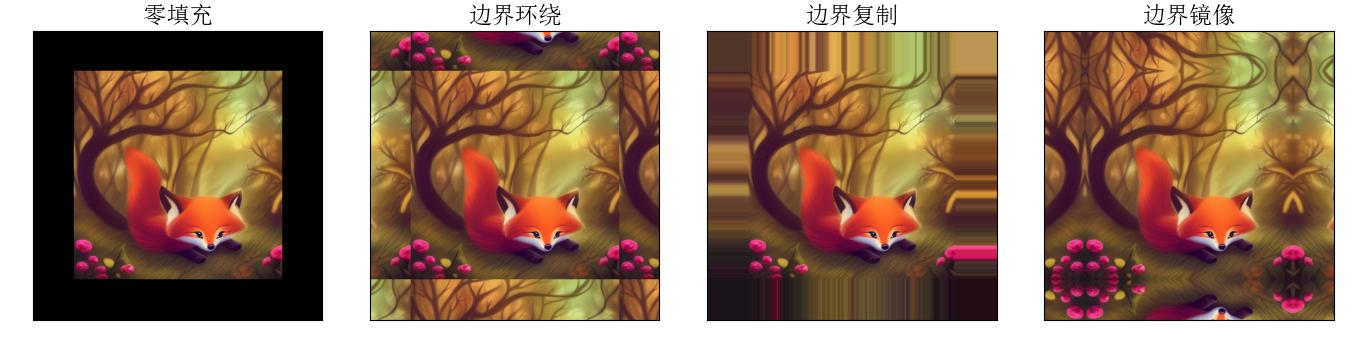
\includegraphics[scale=0.4]{图像填充.png}
\end{figure}

\subsection{Gauss滤波器}

设一维标准差为$\sigma$,均值为$\mu=0$的Gauss函数为$G_{\sigma}(x) = \frac{1}{\sqrt{2\pi}\sigma}\e^{\frac{x^2}{2\sigma^2}}$,
\add 则二维各向同性标准差为$\sigma$且均值$\mu=(0,0)$的Gauss函数为\del
\begin{equation*}
G_{\sigma}(x, y) = G_\sigma(x)G_\sigma(y) = \frac{1}{2\pi\sigma^2}\e^{\frac{x^2+y^2}{2\sigma^2}}
\end{equation*}

\paragraph{Gauss核的大小与标准差关系}由于一维Gauss函数满足3-$\sigma$原则,也就是指密度函数在$|x| < \sigma,2\sigma,3\sigma$上面积分别占比为$68\%,95\%,99.7\%$,
一般取$k=2\sigma$即可,也就是当卷积核大小为$(2k+1)\times(2k+1)$时,取$\sigma = k/2$. Gauss核也就是Gauss函数在$[-k,k]^2$中整数点的差值,
即二维Gauss核为$w_{ij} = G_{k/2}(i-k-1,j-k-1),\ (1\leq i,j\leq 2k+1)$,简记为$G_\sigma$. (注意与Gauss函数区分开,一个是$(2k+1)\times(2k+1)$的矩阵,
另一个是实值函数)

\paragraph{Gauss模糊} 将Gauss核作用在图像上即可得到Gauss模糊(Gaussian Blur)的效果. 设图像为$f$,$\bd{p},\bd{q}$为像素坐标,$f_{\bd{p}}$为图像在$\bd{p}$处的像素值,
卷积核空间为$S_{\bd{p}} = \{\bd{p}+(i,j):(i,j)\in[-k,k]^2\}$(PPT上简记为$S$),则Gauss模糊在$\bd{p}$处的值有以下两种表示方法:
\begin{equation*}
    GB[f]_{\bd{p}} = \sum_{\bd{q}\in S_{\bd{p}}}G_\sigma(||\bd{p}-\bd{q}||)f_{\bd{q}}
    = \sum_{i=-k}^k\sum_{j=-k}^kG_\sigma(||(i,j)||)f(\bd{p}_1+i,\bd{p}_2+j)
\end{equation*}
\textbf{注}:这里$G_\sigma(\cdot)$表示一维Gauss函数. 归一化后的Gauss滤波器表示为以下形式:
\begin{equation*}
    H(\bd{q}) = \frac{1}{W_{\bd{p}}}\e^{-\frac{||\bd{p}-\bd{q}||^2}{2\sigma^2}},\qquad W_{\bd{p}} = \sum_{\bd{q}\in S_{\bd{p}}}\e^{-\frac{||\bd{p}-\bd{r}||^2}{2\sigma^2}}
\end{equation*}

\paragraph{Gauss核的性质}\ \par
1. \textbf{二维Gauss核的可分离性}:设$G_\sigma(x),G_\sigma(x,y)$表示一维和二维Gauss函数,定义与上文相同. 设$2k+1$维的一维Gauss核为
\begin{equation*}
    u = (G_\sigma(-k),G_\sigma(-k+1),\cdots,G_\sigma(0),\cdots,G_\sigma(k-1),G_\sigma(k))^T
\end{equation*}
则二维Gauss核$G_\sigma$满足$G_\sigma = u * u^T$. 利用Gauss核的可分离性,
可以将卷积过程分解为$G_\sigma*f = (u * u^T)*f = u * (u^T * f)$,
从而将时间复杂度由$\O(MN(2k+1)^2)$变为$\O(2MN(2k+1))$.\add

2. \textbf{两个二维Gauss核卷积仍为Gauss核}:设$\sigma^2=\sigma_1^2+\sigma_2^2$,则$(G_{\sigma_1}*G_{\sigma_2})(m,n) = G_{\sigma}(m,n)$.

Gauss核具有平滑图像,起到正则化作用,在图像处理中非常常用,下面是三种基于Gauss核的滤波算子.

\subsubsection{DoG算子}
通过两个不同方差的Gauss函数$G_{\sigma_1},G_{\sigma_2}$,不妨令$\sigma_1 < \sigma_2$,则称$G_{\sigma_1} - G_{\sigma_2}$为$DoG$算子. 
$DoG$算子是一种差分滤波器,本质上是将$G_{\sigma_1}$作用后的图像与$G_{\sigma_2}$作用后的图像做差得到的结果:
\begin{equation*}
    G_{\sigma_1} * f - G_{\sigma_2} * f = (G_{\sigma_1} - G_{\sigma_2})*f
\end{equation*}
\subsubsection{锐化滤波器}
锐化滤波的结果如下:
\begin{align*}
    f_{sharp} =&\ f+\alpha(f-f_{blur}) = (1+\alpha) I\cdot f - \alpha G_{\sigma} * f\\
    =&\ ((1+\alpha)I-\alpha G_\sigma)*f
\end{align*}
则$(1+\alpha)I-\alpha G_\sigma$为锐化滤波器,其中$\alpha$为锐化系数,$I$表示全通滤波器,$3\times 3$的全通滤波器为
\begin{equation*}
I_3 = \left[\begin{matrix}
    0&0&0\\
    0&1&0\\
    0&0&0
\end{matrix}\right]
\end{equation*}
\subsubsection{双边滤波器}  % 重点
Guass模糊只考虑了\textbf{像素坐标距离的关系(空间域,space)},双边滤波器在Gauss模糊的基础上加入\textbf{像素值的关系(值域,range)},从而能对图像边界处有较好的处理.
双边滤波器具有\textbf{保护边缘}的作用,多次重复使用会产生卡通效果,图像变得更加平滑,产生色块.

记图像为$f$,$\bd{p},\bd{q},f_{\bd{p}},S_{\bd{p}},G_{\sigma}$的定义和上述Gauss模糊处的相同,$||\cdot||$表示欧氏距离($\ell_2$范数),$W_p$为归一化系数,
则双边滤波器处理图像$f$后在$\bd{p}$处的结果为
\begin{align*}
    BF[f]_{\bd{p}} =&\ \frac{1}{W_{\bd{p}}}\sum_{\bd{q}\in S_{\bd{p}}}\underbrace{G_{\sigma_s}(||\bd{p}-\bd{q}||)}_{\text{space}}\underbrace{G_{\sigma_{r}}(|f_{\bd{p}} - f_{\bd{q}}|)}_{\text{range}}f_{\bd{q}}\\
    \text{归一化系数:}W_{\bd{p}} =&\ \sum_{\bd{q}\in S_{\bd{p}}}G_{\sigma_s}(||\bd{p}-\bd{q}||)G_{\sigma_{p}}(|f_{\bd{p}} - f_{\bd{q}}|)\\
    \bd{p}\text{处的双边滤波核:}\quad\frac{1}{W_{\bd{p}}}&G_{\sigma_s}(||\bd{p}-\bd{q}||)G_{\sigma_{r}}(|f_{\bd{p}} - f_{\bd{q}}|)
\end{align*}
$G_{\sigma_s}(||\bd{p}-\bd{q}||)$就是方差为$\sigma_s$的Gauss核,$G_{\sigma_{r}}(|f_{\bd{p}} - f_{\bd{q}}|)$是值域做差后再作用Gauss函数得到的核,
对于不同的$\bd{p}$均需要重新计算$G_{\sigma_{r}}(|f_{\bd{p}} - f_{\bd{q}}|)$,而第一部分Gauss核无需重算.

将两个核做内积并归一化处理后,得到在$\bd{p}$处的双边滤波核,再作用于图像$f$上,即可得到$\bd{p}$处的双边滤波结果.
\subsection{其他非线性滤波器}
\paragraph{均值滤波(Mean)}设滤波核的大小为$(2k+1)\times (2k+1)$,滤波结果$g(m,n)$处的值是由图像以$(m,n)$为中心,周围大小为$(2k+1)\times (2k+1)$区域所有值的均值:
\begin{equation*}
    g(m,n) = \frac{1}{(2k+1)^2}\sum_{i=-k}^{k}\sum_{j=-k}^{k}f(m+i,n+j)
\end{equation*}
表示为滤波器的形式为($\bd{p},\bd{q},S_{\bd{p}}$的含义与上文相同,$|S_{\bd{p}}|$表示滤波器的大小)
\begin{equation*}
    H(\bd{q}) = \frac{1}{|S_{\bd{p}}|}
\end{equation*}
\paragraph{阈值滤波(Thresholding)}
设定滤波阈值为$A$,则滤波结果为$g(m,n) = \begin{cases}
    255, &\quad f(m,n) > A,\\
    0,&\quad \text{否则}.
\end{cases}$
\paragraph{整流滤波(Rectification)}
仅保留非负像素,滤波结果为$g(m,n) = \max(f(m,n),0)$. 常用于卷积神经网络中正则化操作.
\paragraph{中值滤波(Median)}
设滤波核大小为$(2k+1)\times(2k+1)$,滤波结果$g(m,n)$处的值是由图像中以$(m,n)$为中心,周围大小为$(2k+1)\times(2k+1)$区域的所有值的中位数,以$k=1$为例:
\begin{equation*}
    g(m,n) = \text{中位数}\left(\left[\begin{matrix}
        f(m-1,n-1)&f(m-1,n)&f(m-1,n+1)\\
        f(m,n-1)&f(m,n)&f(m,n+1)\\
        f(m+1,n-1)&f(m+1,n)&f(m+1,n+1)
    \end{matrix}\right]\right)
\end{equation*}
表示为滤波器的形式为
\begin{equation*}
    H(\bd{q}) = \begin{cases}
        1,&\quad f(\bd{q}) = \mathop{median}_{\bd{q}\in S_{\bd{p}}}\{f(\bd{q})\},\\
        0,&\quad \text{否则}.
    \end{cases}
\end{equation*}

\subsection{Fourier变换}
\begin{definition}[图像的二维Fourier变换与逆变换] 
\add 设图像$f\in \R^{M\times N}$,则
\begin{align*}
    \text{Fourier变换:}&\ \hat{f}(m,n) = \iint_{\R^2}f(x,y)\e^{-2\pi\i\left(\frac{mx}{M}+\frac{ny}{N}\right)}\,\d x\d y\\
    \text{Fourier逆变换:}&\ \check{f}(m,n) = \frac{1}{MN}\iint_{\R^2}f(x,y)\e^{2\pi\i\left(\frac{mx}{M}+\frac{ny}{N}\right)}\,\d x\d y
\end{align*}
Fourier变换也可记为$\F(f) := \hat{f}$,Fourier逆变换$\F^{-1}(f) := \check{f}$.
\end{definition}
\textbf{注}:如果把$\e^{-2\pi\i\left(\frac{mx}{M}+\frac{ny}{N}\right)}$视为$x$轴方向频率为$m/M$的正弦波,与$y$轴方向频率为$n/N$的正弦波叠加形成的二维正弦波,
则$\hat{f}(m,n)$可以视为图像$f$在复合波上的投影,\textbf{Fourier变换是空域(空间域)到频域的映射},并且$\hat{f}(m,n)$的\underline{辐角表示该种正弦波的相位大小},$|\hat{f}(m,n)|$表示\underline{该种正弦波辐角大小}.
\textbf{高频}部分($m,n$偏大)存储图像的细节信息,\textbf{低频}部分($m,n$偏小)存储图像的轮廓信息.

\paragraph{Fourier变换关于卷积的性质}\ \par
设图像$f,g\in \R^{M\times N}$,在两个图像维数相同前提下,定义图像的\textbf{点积(内积)}$f\cdot g$为$(f\cdot g)(m,n) := f(m,n)g(m,n)$,即对应元素相乘.
下面定理说明\textbf{Fourier变换将空域的卷积转化为频域的点积},\textbf{Fourier逆变换将频域的卷积转化为空域的点积}.
\add

1. 空间域卷积定理:$\wdh{f*g} = \hat{f}\cdot \hat{g}$.\add

2. 频域卷积定理:$\F^{-1}(\hat{f}*\hat{g}) = a(f\cdot g)$,其中常数$a = MN$.
\subsection{图像参数化几何变换}\label{sec-二维几何变换}

1. 平移变换(自由度为$2$)
\begin{equation*}
    \bd{x}' = \bd{x}+\bd{t}\iff \bd{x}' = \left[\begin{matrix}
        1&0&t_1\\ 0&1&t_2\\ 0&0&1
    \end{matrix}\right]\left[\begin{matrix}
        x_1\\x_2\\1
    \end{matrix}\right],\ \text{逆矩阵为}\ \left[\begin{matrix}
        1&0&-t1\\0&1&-t2\\0&0&1
    \end{matrix}\right].
\end{equation*}

2. 旋转变换(自由度为$1$)
\begin{equation*}
    \bd{x}' = R_{\theta}\bd{x}\iff \bd{x}' = \left[\begin{matrix}
        \cos\theta&-\sin\theta&0\\
        \sin\theta&\cos\theta&0\\
        0&0&1
    \end{matrix}\right]\left[\begin{matrix}
        x_1\\x_2\\1
    \end{matrix}\right],\ \text{逆矩阵为}\ \left[\begin{matrix}
        \cos\theta&\sin\theta&0\\
        -\sin\theta&\cos\theta&0\\
        0&0&1
    \end{matrix}\right].
\end{equation*}

3. 欧式变化(自由度为$3$)
\begin{equation*}
    \bd{x}' = [R_\theta|\bd{t}]\bd{x}\iff \bd{x}' = \left[\begin{matrix}
        \cos\theta&-\sin\theta&t_1\\
        \sin\theta&\cos\theta&t_2\\
        0&0&1
    \end{matrix}\right]\left[\begin{matrix}
        x_1\\x_2\\1
    \end{matrix}\right],\ \text{逆矩阵为}\ \left[\begin{matrix}
        \cos\theta&\sin\theta&-t_1\cos\theta-t_2\sin\theta\\
        -\sin\theta&\cos\theta&t_1\sin\theta-t_2\cos\theta\\
        0&0&1
    \end{matrix}\right].
\end{equation*}

4. 相似变换(自由度为$4$)
\begin{equation*}
    \hspace*{-1.6cm}\bd{x}' = [R_\theta|\bd{t}]\bd{x}\iff \bd{x}' = \left[\begin{matrix}
        s\cdot \cos\theta&-s\cdot\sin\theta&t_1\\
        s\cdot \sin\theta&s\cdot \cos\theta&t_2\\
        0&0&1
    \end{matrix}\right]\left[\begin{matrix}
        x_1\\x_2\\1
    \end{matrix}\right],\ \text{逆矩阵为}\ \left[\begin{matrix}
        \frac{1}{2s}\cdot \cos\theta&\frac{1}{2s}\cdot\sin\theta&\frac{-t_1\cos\theta-t_2\sin\theta}{s}\add \\
        -\frac{1}{2s}\cdot \sin\theta&\frac{1}{2s}\cdot \cos\theta&\frac{t_1\sin\theta-t_2\cos\theta}{s}\\
        0&0&1
    \end{matrix}\right].
\end{equation*}

5. 仿射变换(自由度为$6$)
\begin{equation*}
    \bd{x}' = \bd{x}+\bd{t}\iff \bd{x}' = \left[\begin{matrix}
        a_{11}&a_{12}&t_1\\
        a_{21}&a_{22}&t_2\\
        0&0&1
    \end{matrix}\right]\left[\begin{matrix}
        x_1\\x_2\\1
    \end{matrix}\right].
\end{equation*}

\subsection{前向变换与逆向变换}
设变换矩阵为$T$,原图像记为$f$,变换后的图像记为$g$,则对于图像中每个像素坐标$\bd{x}$满足
\begin{equation*}
    g(T\bd{x}) = f(\bd{x}),\qquad g(\bd{x}) = f(T^{-1}\bd{x}).
\end{equation*}
其中,前者为\textbf{前向变换(forward warping)},后者为\textbf{逆向变换(inverse warping)}. 

前向变换中,由于$\bd{x}$的参数为整数,而$T\bd{x}$不一定为整数,所以填充时会出现空缺部分;
而逆向变换中,计算$T^{-1}\bd{x}$非整数时,可通过内插算法获得该像素处的近似值,可以很好解决空缺问题.

\subsection{图像内插}
注意将图像内插与上采样区分开,图像内插是一种\textbf{一般的插值},可在任意位置处插值,而上采样一般按照$2$的倍数插值.

内插方法:设原图像大小为$M\times N$,记为$f(x,y),\ x\in[1,M],y\in[1,N]$,考虑二维平面中非整数点$(x^*, y^*)$,一种求解$f(x^*,y^*)$的方法.
(也即将$f$延拓到$\R^2$中)

\textbf{近邻插值}:使用原图中距离$(x^*,y^*)$最近的像素进行代换:
\begin{equation*}
 (x_0,y_0) = \argmin_{(x,y)\in[1,M]\times[1,N]\cap \N^2}||(x,y)-(x^*,y^*)||_2,
\end{equation*}
其中$||\cdot||_2$表示$\ell_2$范数,则$f(x^*,y^*) = f(x_0,y_0)$.

\textbf{双线性插值}:将$(x^*,y^*)$与周围整数点所围成的面积反比作为整数点对应像素的加权值,
设$O(x^*,y^*)$周围存在四个整数点$A(x_h, y_h),\ B(x_h, y_l),\ C(x_l, y_l),\ D(x_l, y_h)$,
对应的面积分别为$S_A = S(O,C),\ S_B = S(O, D),\ S_C = S(O, A),\ S_D = S(O, B)$,
其中$S(O,A)$表示由点$O,A$所围成的面积,参考右图. 则有\del\del

{\begin{wrapfigure}[10]{r}{.3\linewidth} % 文字环绕行数为13行, 图片靠右 (l为靠左), 图片占0.5的行宽
    \centering
    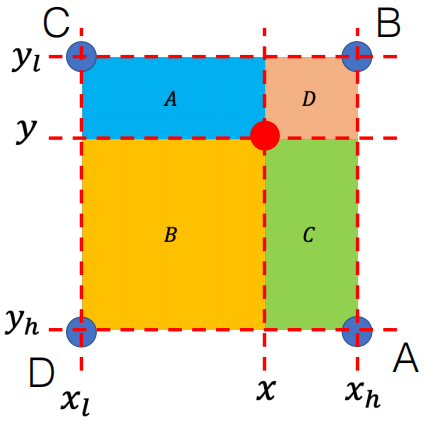
\includegraphics[scale=1.2]{双线性插值.png}
    \caption{双线性插值}
\end{wrapfigure}
\begin{equation*}
    f(x^*, y^*) = S_Af(A)+S_Bf(B)+S_Cf(C)+S_Df(D).
\end{equation*}}
\vspace{2cm}
\subsection{下采样与上采样}  % 重点
\subsubsection{下采样(subsample)}
\begin{definition}[下采样定理,Shannon-Nyquist 定理]
    设每隔$p$个像素进行一次采样,则采样频率为$1/p$,图像中像素的最高频率为$f_{max}$,当$1/p > 2f_{max}$时,采样后的图像保留了原始图像的全部信息.
\end{definition}
在图像处理中,如果采样频率较低,则会出现混淆的问题,无法保留图像全部特征. 采样定理告诉我们,对于给定的采样频率,可以通过降低图像中的最高频率从而提高采样效果,
也就是对原图像做平滑处理,最常用的就是Gauss模糊.

\paragraph{下采样步骤}先对原图像做Gauss模糊,然后做间距为$p$的等距插值即可获得下采样结果.

\paragraph{Gauss金字塔}
若原图像大小为$2^k\times 2^k$,间距为$2$的下采样得到的图像大小为$2^{k-1}\times 2^{k-1},\cdots,4\times 4,2\times 2,1\times 1$,
将其分别记为$G_0,G_1,\cdots,G_k$,其中$G_0$为原图像,$G_i,\ (i \geq 1)$是原图像等距离缩小$2^i$倍的下采样结果,将$\{G_i\}$称为\textbf{Gauss金字塔}.

Gauss金字塔的一个应用是\textbf{基于滑动窗口的模板匹配},将每次缩放结果$G_i$中用滑动窗口搜索目标模板,可通过互相关计算相似度,当相似度超过一定阈值时,
则认为匹配到目标,然后将匹配到的滑动窗口重新放大$2^i$倍,则可得到原始图像中匹配的滑动窗口位置,对应了原始图像中的目标位置.

\subsubsection{上采样(upsample)}
上采样分为以下三步:
\begin{enumerate}
    \item 用$0$填充图像(若放大倍数为$2$,则在每行的左侧用$0$对图像进行填充,列也是相同操作)
    \item 在填充后的图像上进行Gauss模糊.
    \item 由于像素值填充了大量的$0$,所以需要对图像亮度进行整体提高.
\end{enumerate}
\paragraph{Laplace金字塔}记上采样操作为$\text{expand}(\cdot)$,原图为$G_0$,$n$次得到的下采样结果为$\{G_1,\cdots,G_n\}$,
则$n$层Laplace金字塔构造过程为
\begin{align*}
    L_0 =&\ G_0 - \text{expand}(G_1),\\
    L_1 =&\ G_1 - \text{expand}(G_2),\\
    \vdots\ &\\
    L_n =&\ G_n
\end{align*}
将$\{L_i\}$称为\textbf{Laplace金字塔},$L_i,\ (i < n)$的计算方式为:将原图像$G_{i}$做下采样得到$G_{i+1}$,再与$G_{i+1}$上采样结果$\text{expand}(G_{i+1})$做差,
即可得到$L_i$.

\textbf{用途}:为了存储图像$G_0$,可以仅存储图像内容更少的$\{L_i\}$,从而节约内存,可通过递归执行上采样获得原始图像:
\begin{equation*}
    G_0 = L_0+\text{expand}(L_1+\text{expand}(L_2+\text{expand}(\cdots+\text{expand}(L_n))))
\end{equation*}

\textbf{性质}:当图像很小、距离远时,主要观察到\textbf{低频信息};当图像很大、距离近时,同时能观察到\textbf{高频和低频信息}.

\section{图像特征提取}
总共有三种特征:边缘特征,角点特征,斑点特征.
\subsection{边缘检测}
图像中边缘出现的位置有以下$6$个:
\begin{enumerate}
    \item 亮度有巨大改变;
    \item 角点、交叉点;
    \item 景深的不连续处(前景与背景深度的不同);
    \item 曲面法向量的不连续处(例如正方体的棱);
    \item 物体表面反射率不同(例如物体表面有不同的颜色);
    \item 物体阴影边缘.
\end{enumerate}

\subsubsection{图像微分}
在图像中,用差值近似图像微分,由于存在$x,y$两个方向,所以也就是求图像像素梯度,先要求出每个像素点在$x,y$方向上的偏导数,然后表示为向量的形式:
\begin{align*}
    x\text{方向偏导数:}&\ \frac{\partial f}{\partial x}(x, y)\approx f(x+1,y) - f(x,y)\\
    y\text{方向偏导数:}&\ \frac{\partial f}{\partial y}(x, y)\approx f(x,y+1) - f(x,y)\\
    \text{图像微分:}&\ \nabla f(m, n) = \left[\frac{\partial f}{\partial x}(m,n),\frac{\partial f}{\partial y}(m,n)\right]
\end{align*}
则可以计算出每个像素处的幅度(范数)和辐角:
\begin{equation*}    
||\nabla f||(m,n) = \sqrt{f_x(m,n)^2+f_y(m,n)^2},\quad \theta(m,n) = \arctan\left(\frac{f_y(m,n)}{f_x(m,n)}\right).
\end{equation*}
但图像噪声对直接微分的结果影响非常大,所以需要先用Gauss模糊对图像进行平滑处理.
\paragraph{Gauss微分核}对Gauss核做微分后得到的结果,相当于先对图像做平滑处理,再求偏导数:
\begin{equation*}
    \frac{\partial}{\partial x}(G_\sigma * f) = (\frac{\partial}{\partial x}G_\sigma)*f
\end{equation*}

\paragraph{各向异性Gauss微分核}由于默认的Gauss核是各向同性的,也就是在$x,y$方向上的变化率均相同,这是因为将二维Gauss分布中$\sigma_1,\sigma_2$设置为相同;
如果令$\sigma_1 \gg \sigma_2$,则表示几乎不对$x$方向进行平滑处理,仅对$y$方向进行平滑处理. 再对其求偏导数,得到各向异性Gauss微分核.

\paragraph{Sobel微分核}这是一种各向异性Gauss微分核的特例,仅在$y$(或者$x$)方向上作平滑处理,在$x$(或者$y$)方向上求偏导:
\begin{equation*}
    S_x = \left[\begin{matrix}
        1\\2\\1
    \end{matrix}\right]*\left[\begin{matrix}
        1&0&-1
    \end{matrix}\right] = \left[\begin{matrix}
        1&0&-1\\
        2&0&-2\\
        1&0&-1
    \end{matrix}\right],\ 
    S_y = \left[\begin{matrix}
        1\\0\\-1
    \end{matrix}\right]*\left[\begin{matrix}
        1&2&1
    \end{matrix}\right] = \left[\begin{matrix}
        1&2&1\\
        0&0&0\\
        -1&-2&-1
    \end{matrix}\right]
\end{equation*}
\subsection{Canny边缘检测}  % 重点
Canny边缘检测算法共分为以下三步(PPT上为四步,将第一步分为求偏导和求梯度两步):

\textbf{1. 梯度提取},取方差为 \(\sigma\)
的Gauss一阶微分核做卷积,得到幅度图和辐角图.

\textbf{2. 非极大值像素梯度抑制(Non-Maximum Suppression,NMS)},对每个像素考虑其梯度方向上的两个临近点,
用\textbf{双线性插值}获得两点处的梯度值,然后判断中间点的梯度范数是否大于两端的梯度范数,若大于则保留,反之舍弃(归零).

具体来讲,设当前像素点为 \(\boldsymbol{q}= (x, y)\), 幅度图记为
\(||\nabla f||(x, y)\),\(\boldsymbol{q}\) 点处的梯度方向记为
\(\theta\),则考虑沿梯度方向上的两点

\[\boldsymbol{r}:(x+\cos \theta, y+\sin\theta),\quad
\boldsymbol{p}=(x-\cos\theta, y-\sin\theta)\]

若
\(||\nabla f||(\boldsymbol{q}) > \max\bigg\{||\nabla f||(\boldsymbol{r}),||\nabla f||(\boldsymbol{p})\bigg\}\),则保留该点,否则令
\(f(\boldsymbol{q}) = 0\).\add

\textbf{3. 滞后阈值处理,边缘连接(Hysteresis thresholding, Boundary)},考虑对NMS结果进一步处理,设定高阈值和低阈值.
我们称所有幅度值\textbf{大于高阈值}的点为\textbf{高阈值点},所有幅度值\textbf{大于低阈值}的点为\textbf{低阈值点}.
每次从高阈值点开始绘制边缘,寻找周围低阈值点进行连接,若当前点附近仍有低阈值点则继续连接,直到连接完全部的高阈值点后,得到的就是Canny边缘处理结果.

\subsection{Harris角点检测}  % 重点
设图像为$I(\cdot\, ;\cdot)$,考虑一个大小为$(2k+1)\times (2k+1)$中心位于$\bd{x}_0\in\R^2$的滑动窗口$W_k(\bd{x}_0)$,
任取一个滑动方向$\bd{t}\in\R^2$,定义在$\bd{t}$方向上的\textbf{平方误差和(Sum up Squared Differences, SSD)}为
\begin{equation*}
    E_{\bd{x}_0}(\bd{t}) = \sum_{\bd{x}\in W_k(\bd{x}_0)}\left(I(\bd{x}+\bd{t})-I(\bd{x})\right)^2
\end{equation*}
若$\bd{x}_0$为角点,则$\forall \bd{t}\in\R^2$,$E_{\bd{x}_0}(\bd{t})$都应尽可能大.

记$\bd{t} = (u,v)^T$,由Taylor公式可知
\begin{equation*}
    I(\bd{x} + \bd{t}) = I(\bd{x}) + I_x(\bd{x})u+I_y(\bd{x})v+O(||\bd{t}||_2^2)
\end{equation*}
于是可对$E_{\bd{x}_0}(\bd{t})$进行进一步分解
\begin{align*}
    E_{\bd{x}_0}(\bd{t})\approx&\  \sum_{x\in W_k(\bd{x}_0)}\left(I(\bd{x}) + I_x(\bd{x})u+I_y(\bd{x})v-I(\bd{x})\right)^2\\
    =&\ \sum_{\bd{x}\in W_k(\bd{x}_0)}\left(I_x(\bd{x})u+I_y(\bd{x})v\right)^2.
\end{align*}

更一般的,设图像$I$大小为$M\times N$,记全体像素点集为$D:=[1,M]\times [1,N]\cap \Z^2$,则
\begin{align*}
    E_{\bd{x}_0}(\bd{t})\approx&\ \sum_{\bd{x}\in D}w_{\bd{x}_0}(\bd{x})\left(I_x(\bd{x})u+I_y(\bd{x})v\right)^2\\
    =&\ \sum_{\bd{x}\in D}w_{\bd{x}_0}(\bd{x})I_x^2(\bd{x})u^2+ 2w_{\bd{x}_0}(\bd{x})I_x(\bd{x})I_y(\bd{x})uv+w_{\bd{x}_0}(\bd{x})I_y^2(\bd{x})v^2\\
    =&\ A(\bd{x}_0)u^2+2B(\bd{x}_0)uv+C(\bd{x}_0)v^2.
\end{align*}
其中$w_{\bd{x_0}}(\bd{x}) = \begin{cases}
    1,&\quad \bd{x}\in W_k(\bd{x}_0),\\
    0,&\quad \texttt{otherwise}.
\end{cases}$为$W_k(\bd{x}_0)$的示性函数,\add 为使其变化更平滑,可取$w_{\bd{x}_0}$为中心在$\bd{x}_0$大小为$(2k+1)\times (2k+1)$的Gauss核,上式中$A,B,C$定义如下,分别表示将核$w$作用在$I_x^2,\ I_xI_y,\ I_y^2$图像上得到的结果
\begin{equation*}
A(\bd{x_0}) = \sum_{x\in D}w_{\bd{x}_0}(\bd{x})I_x^2(\bd{x}),\ B(\bd{x_0}) = \sum_{x\in D}w_{\bd{x}_0}(\bd{x})I_x(\bd{x})I_y(\bd{x}),\ C(\bd{x_0}) = \sum_{x\in D}w_{\bd{x}_0}(\bd{x})I_y^2(\bd{x}).
\end{equation*}
进一步,可使用二次型矩阵表出
\begin{equation*}
    E_{\bd{x}_0}(\bd{t}) = \bd{t}^TM_{\bd{x}_0}\bd{t},\quad \text{其中 }M_{\bd{x}_0}=\left[\begin{matrix}
        A(\bd{x_0})&B(\bd{x}_0)\\
        B(\bd{x_0})&C(\bd{x}_0)\\
    \end{matrix}\right]
\end{equation*}
称$M_{\bd{x}_0}$为图像在$\bd{x}_0$处的\textbf{二阶矩矩阵(Second moment matrix)}.

假设$M_{\bd{x}_0}$的秩为$2$,则$M_{\bd{x}_0}$存在$2$个特征值,记其中较大者为$\lambda_{max}$,较小者为$\lambda_{min}$,
对应的特征向量分别为$\bd{x}_{max},\ \bd{x}_{min}$,由特征向量定义可知,
$M_{\bd{x}_0}\bd{x}_{max} = \lambda_{max}\bd{x}_{max}$说明窗口$W_k(\bd{x}_0)$在沿着$\bd{x}_{max}$方向上移动单位长度可使得
$E_{\bd{x_0}}(\bd{t})$达到最大值. 下面对$\lambda$的大小进行分类讨论

1. 当$\lambda_{max}$较小时,$E_{\bd{x_0}}(\bd{t})$沿各个方向变化都较小,则$\bd{x}_0$处于图像内部平滑区域.

2. 当$\lambda_{max}$较大且$\lambda_{max}\approx\lambda_{min}$时,$E_{\bd{x_0}}(\bd{t})$沿各个方向变化都较大,则$\bd{x}_0$是角点.

3. 当$\lambda_{max}$较大且$\lambda_{max}\gg\lambda_{min}$时,$E_{\bd{x_0}}(\bd{t})$仅沿$\bd{x}_{max}$方向变化较大,则$\bd{x}_0$是边界点.

通过引入\textbf{角点响应函数(Corner response function)}用于判断角点
\begin{align*}
    R(\bd{x}_0) =&\ \det(M_{\bd{x}_0}) - \alpha\cdot\text{trace}(M_{\bd{x}_0})^2 = \lambda_1\lambda_2 - \alpha(\lambda_1+\lambda_2)^2\\
    =&\ A(\bd{x_0})C(\bd{x_0}) - B^2(\bd{x_0}) - \alpha(A(\bd{x_0})+C(\bd{x_0}))
\end{align*}
其中$\alpha\in[0.04,0.06]$为超参数. 当$R(\bd{x}_0)$大于设定阈值时,则判定$\bd{x}_0$为角点. 响应函数与特征值关系可参考右图:\vspace{-1cm}

\begin{wrapfigure}[8]{r}{.4\linewidth} % 文字环绕行数为13行, 图片靠右 (l为靠左), 图片占0.5的行宽
    \hspace{-1.4cm}
    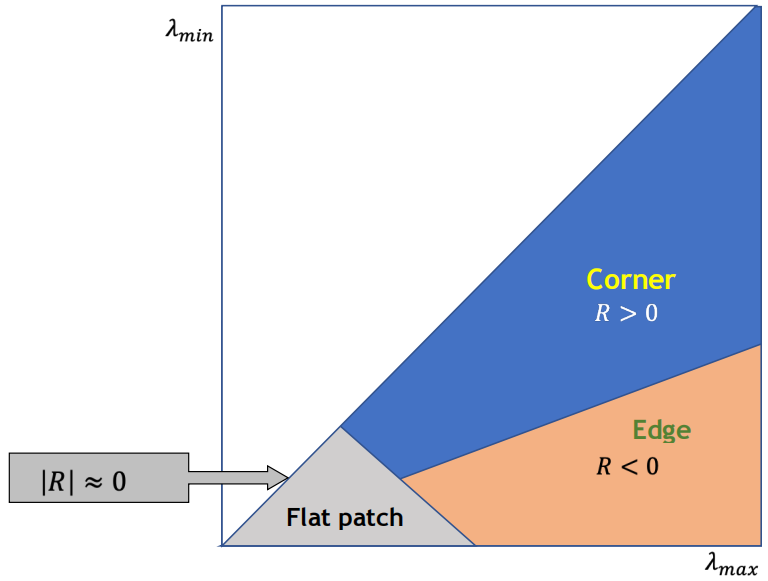
\includegraphics[scale=0.5]{Harris角点相应函数.png}
\end{wrapfigure}
\ \vspace{1cm}

最后,再使用\textbf{非局部极大值抑制(Non-maxima suppression, NMS)},
若$\bd{x}_0$是其邻域内的最大值,则对其进行保留,否则删去该点. 通过设定邻域大小,可对角点密度进行调整.

整个Harris角点检测算法中,总共存在4个超参数,分别为窗口大小$k$,响应函数中的$\alpha$,响应阈值和NMS邻域大小.

\paragraph{Harris角点检测的等变性、不变性和特异性}\ \par
角点检测中存在两个讨论对象:一个是\textbf{角点位置},另一个是\textbf{角点检测}(是否角点,取决于特征值、响应函数的变换).

1. 等变性:\textbf{角点位置}的平移等变性、旋转等变性、缩放等变性.

2. 不变性:\textbf{角点检测}的平移不变性、旋转不变性,\textbf{角点位置和角点检测}对整体光强\textbf{增加常数}的不变性.

3. 特异性:整体光强\textbf{按倍数缩放}会导致角点检测失效(例如修改对比度),\textbf{缩放图像}也会导致检测失效.

\textbf{平移图像}:由于平移图像只会导致角点位置发生改变,所以角点位置对平移变换具有等变性;特征值是基于微分计算的,所以平移不会对特征值产生影响,
由于响应函数取决于特征值,故角点检测是不变的.

\textbf{旋转图像}:由于旋转图像也会导致角点位置发生改变,所以角点位置对平移变换具有等变性;由于图像旋转,相当于检测框进行了旋转,所以只会对特征向量
的方向进行旋转,特征值保持不变,由于响应函数取决于特征值,故角点检测是不变的.

\textbf{光强缩放导致角点检测失效的原因}:设图像为$I$,光强变换后为$I' = aI+b$,将全部像素值缩放$a$倍,增加常数$b$,
则偏导数会变为$I'_x = aI_x,\ I'_y = aI_y$,
二阶矩矩阵$M' = a^2M$,则特征值变化为$\lambda_i' = a^2\lambda_i'$,响应函数变化为$R' = a^2R$,由于阈值与之前相同,
如果$a<1$,则原来可检测到的角点,可能因为响应值降低,导致无法检测到,或者$a>1$,导致检测到很多错误角点,所以按倍数缩放光强会导致角点检测错误.

\textbf{缩放导致角点检测失效的原因}:将图片放大,而检测窗口大小没有增大,由于所有的角点周围的边都被放大,角点框对应的变化幅度降低,
导致\textbf{将角点识别为边},无法检测出角点.

\textbf{解决图像缩放失效的方案}:本质是无法确定图像最适合的检测窗口大小,所以尝试各种不同的检测窗口大小,在人工标定的角点处进行检测,
选取响应值最高的窗口大小.
\subsection{斑点特征}
\textbf{斑点特征(blob)}是圆圈形状的\textbf{特征区域},可以通过\textbf{Laplacian算子:LoG(Laplacian of Gaussian)核}或者DoG核可以找到. LoG核为
\begin{equation*}
    \nabla^2G_\sigma = \frac{\partial G_\sigma^2}{\partial x^2}+\frac{\partial G_\sigma^2}{\partial y^2}
\end{equation*}
LoG核的效果类似于将DoG核取相反数,将标准差大的Gauss核与标准差小的Gauss核做差得到.

通过对图像作用不同的标准差$\sigma$大小,取卷积后图像中的\textbf{局部极大值或局部极小值}作为斑点圆心$(x,y)$,斑点半径$r$与$\sigma$正相关,
一般取为$\sqrt{3}\sigma$(可通过求Laplacian算子的极大值点得到). 可以将一个斑点记为$(x,y,r)$,作为图像的特征区域.

\textbf{特征尺度}:特征区域的大小,可以用斑点半径大小来衡量.  % 待讨论
\subsection{特征描述子}
将图像中的\textbf{关键点}(如角点)或\textbf{区域}(如边缘、斑点)转换为对应的\textbf{特征信息},
对应的关键点的特征信息称为\textbf{特征描述子(Feature descriptor)},一般为向量形式,
特征描述子应该具有以下两个性质:
\begin{itemize}
    \item \textbf{不变性(Invariance)}:图像变换后,对应关键点的特征描述子之间的距离变换很小.(此处的距离一般指欧氏距离或互相关大小)
    \item \textbf{判别性(Discriminability)}:每个关键点的特征描述子应具有较高的唯一性.(与其他关键点的特征描述子距离较远)
\end{itemize}
\subsubsection{相似性衡量} 设描述子向量为$\bd{x},\bd{y}$,则对$\bd{x},\bd{y}$有如下两种常用的衡量方式:
\begin{enumerate}
    \item \textbf{SSD(欧氏距离,Sum up Squared Different)}:$d(x,y) = ||\bd{x}-\bd{y}||_2^2$;
    \item \textbf{NCC(归一化互相关,Normalized Cross Correlation)}:可将归一化分为以下两步
    \begin{enumerate}
        \item 减去均值:$x' = x-\text{mean}(x)$;($\text{mean}(\bd{x})$表示取向量$x$中每个元素的均值)
        \item 单位化:$x'' = \frac{x}{||x||_2}$
    \end{enumerate}
    则$d(x,y) = \bd{x}\cdot \bd{y}$.(向量的点积就是互相关)
\end{enumerate}
\subsubsection{常用特征描述子}
\textit{(由于在考试内容中未提及,仅列出概述)}

1. \textbf{MOPS(多尺度定向窗口描述子,Multiscale Oriented PatcheS descriptor)}:以角点作为关键点,采用固定窗口大小搜索角点,
并使窗口方向与角点的最大特征值对应的特征向量保持一致,对不同尺度大小的图片得到多个窗口. 由于每个角点对应一个窗口,所以窗口内的信息就是该角点对应的描述子.

缺点:由于角点检测受光强影响,所以无法检测不同光照环境下的物体.

2. \textbf{SIFT(尺度不变特征转换,Scale Invariant Feature Transform)}:以斑点作为关键区域,用边的特征构造描述子. 采用DoG检测特征尺度,
将每个斑点划分为网格状,对每个网格统计全部像素点的梯度直方图(将梯度离散化),确定网格中主要梯度方向,最后将梯度主要梯度方向,网格化梯度信息
作为对应斑点的描述子.

优点:由于按照梯度直方图进行划分,所以对于微小形变,描述子在梯度方向上具有不变性;又由于按照网格进行划分,对于微小形变,描述子在空间上也具有不变性.

\subsubsection{图像对齐}\label{sec-图像对齐}
对于两幅图像$f,g$,假设$g$是$f$通过形变$T$得到的,即$Tf = g$,需要反向求出形变矩阵$T$的具体参数值:
\begin{enumerate}
    \item 检测图像关键点(区域);
    \item 计算每个关键点(区域)的特征描述子;
    \item 选择图$f$中的特征描述子与图$g$中每个特征描述子进行比较,选择最相似的一对;
    \item 对于图$f$中每个特征描述子重复上述步骤$3$;
    \item 对最优点对集合,用最小二乘法求解形变矩阵$T$.
\end{enumerate}
其中变换矩阵的参数形式有以下两种:

1. 仿射矩阵(Affine,二维),总计$6$个参数,表示为如下形式:
\begin{equation*}
    T = \left[\begin{matrix}
    a_{11}&a_{12}&a_{13}\\
    a_{21}&a_{22}&a_{23}\\
    0&0&1
    \end{matrix}
    \right]
\end{equation*}

2. 单应性矩阵(Homography,三维),总计$8$个参数,表示为如下形式:
\begin{equation*}
    H = \left[\begin{matrix}
    h_{11}&h_{12}&h_{13}\\
    h_{21}&h_{22}&h_{23}\\
    h_{31}&h_{32}&1
    \end{matrix}
    \right]
\end{equation*}
\paragraph{构造求解单应性矩阵的参数方程}设一个点对为$\bd{x} = (x,y)$和$\bd{x}'' = (x'',y'')$,则
\begin{equation*}
    \left[\begin{matrix}
        h_{11}&h_{12}&h_{13}\\
        h_{21}&h_{22}&h_{23}\\
        h_{31}&h_{32}&1
    \end{matrix}\right]
    \left[\begin{matrix}
        x\\y\\1
    \end{matrix}\right] = 
    \left[\begin{matrix}
        x'\\y'\\z'
    \end{matrix}\right]\qquad
    \frac{1}{z'}\left[\begin{matrix}
        x'\\y'\\z'
    \end{matrix}\right] = \left[\begin{matrix}
        x''\\y''\\1
    \end{matrix}\right]
\end{equation*}
用矩阵表示为$\bd{x}' = H\bd{x},\bd{x}'' =\frac{1}{z'}\bd{x}'$,则对于$H$中的参数应有如下方程满足:
\begin{equation*}
    \begin{cases}
        x'' = \frac{h_{11}x+h_{12}y+h_{13}}{h_{31}x+h_{32}y+1},\add\\
        y'' = \frac{h_{21}x+h_{22}y+h_{23}}{h_{31}x+h_{32}y+1},\\
    \end{cases}\Rightarrow
    \begin{cases}
        h_{11}x+h_{12}y+h_{13} - x''h_{31}x-x''h_{32}y - x'' = 0,\\
        h_{21}x+h_{22}y+h_{23} - y''h_{31}x-y''h_{32}y - y'' = 0.
    \end{cases}
\end{equation*}
描述为矩阵的形式就是(下面虚线部分表示其他点对的数据)
\begin{equation*}
    \left[\begin{matrix}
        x&y&1&0&0&0&-x''x&-x''y&-x''\\
        0&0&0&x&y&1&-y''x&-y''y&-y''\\
        \vdots&\vdots&\vdots&\vdots&\vdots&\vdots&\vdots&\vdots&\vdots
    \end{matrix}\right]\left[\begin{matrix}
        h_{11}\\h_{12}\\h_{13}\\h_{21}\\h_{22}\\h_{23}\\h_{31}\\h_{32}\\1
    \end{matrix}\right] = \left[\begin{matrix}
        0\\0\\\vdots
    \end{matrix}\right]
\end{equation*}
由该方程可以发现,一个点对可以确定$2$个方程,总共有$8$个待定参数,所以至少需要$4$个点对才能确定单应性矩阵$H$. 
当点对数目超过$4$个时,可以使用最小二乘法求解参数.

\subsubsection{RANSAC算法}  % 重点
在上述图像对齐的第$5$步中的最优点对集合中,由于噪声干扰,有可能存在异常值点,通过RANSAC算法可以排除掉这些异常值点.

以二维点对集合$S$为例,设$n=2$表示随机选取点的个数,设定可容许范围大小为$\varepsilon$,假设集合$S$中正常值的占比为$w$,迭代算法$k$次,每次迭代具体操作为:
\begin{enumerate}
    \item 从点集合$S$中随机选取$2$个点,并由这两个点构成直线$l$.(高维空间中则是超平面)
    \item 将集合$S$中到$l$的距离不超过$\varepsilon$的点称为内点(inlier point),否则称为外点(outlier point).
    \item 若当前内点数目大于之前迭代的最大内点数目,则将当前的内点集合替换之前的最优内点集合.
    \item 重复步骤1到3,总计$k$次.
\end{enumerate}
下面用概率的方式,利用假设的正常值占比$w$,可以推导$k$适合的取值大小:
\begin{itemize}
    \item 随机选的点中全是正常值的概率为$w^n$;
    \item 随机选的点中至少有一个是异常值的概率为$1-w^n$;
    \item 进行$k$次迭代,每次选中的点中都至少有一个异常值的概率为$(1-w^n)^k$;
    \item 进行$k$次迭代,存在一次选中的点中全为正常值的概率为$p=1-(1-w^n)^k$.
\end{itemize}
于是我们取定$p=0.99$,也就是说由$99\%$的把握认为,RANSAC算法可以取到至少$n$个正常点. 于是可以计算出不同$w$值和$n$下的迭代次数$k$至少取多大(列为异常值占比$1-w$):
\begin{figure}[htbp]
    \centering
    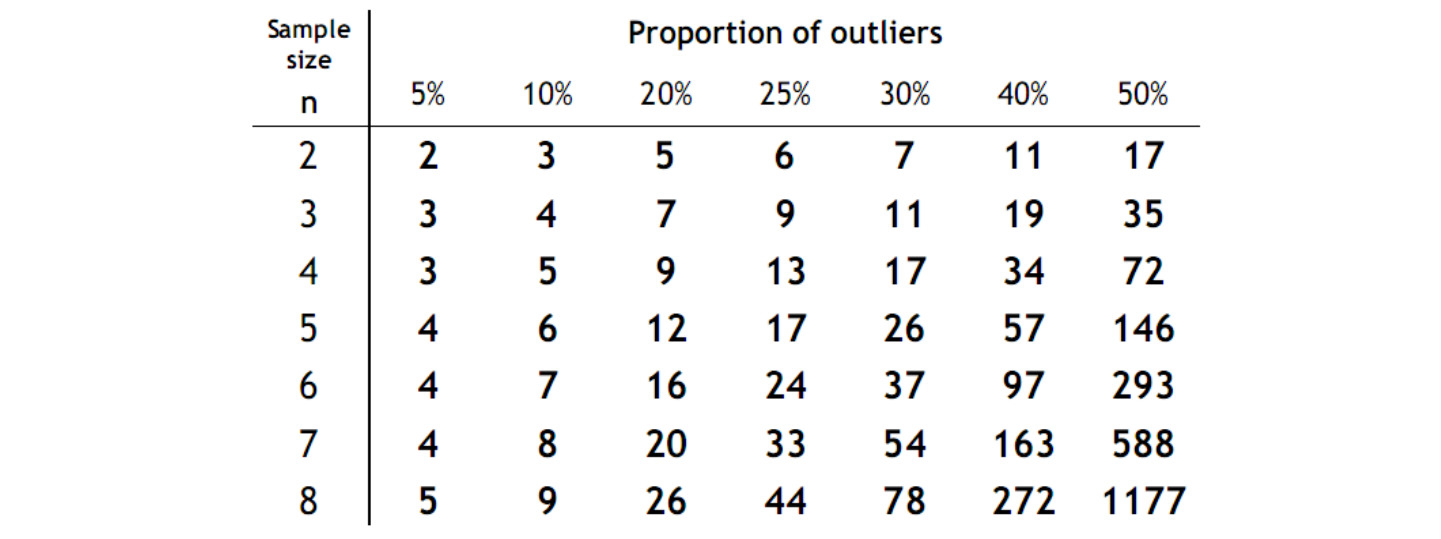
\includegraphics[scale=0.4]{RANSAC迭代次数取值.png}
\end{figure}
\paragraph{迭代RANSAC(Iteratial RANSAC)} 在RANSAC得到的最优内点集$D$基础上进一步优化内点集:
\begin{enumerate}
    \item 用最小二乘法求解通过当前内点集$D$的超平面.
    \item 根据超平面重新寻找内点集$D'$.
    \item 若$D\neq D'$,则$D\leftarrow D'$,回到第一步;否则退出迭代,返回最后得到的内点集$D$.
\end{enumerate}
\paragraph{估计单应性矩阵} 在图像对齐得到的最优点对集合$S$基础上,求解单应性矩阵$H$:
\begin{enumerate}
    \item 随机选取$4$个点对;(求解$H$所需的最少点对数目)
    \item 计算单应性矩阵$H$;(列出参数方程,最小二乘法求解)
    \item 当$||\bd{x}_i-H\bd{x}_i'||_2^2 < \varepsilon,\ (\bd{x}\in S)$时,认为$\bd{x}$是内点;
    \item 重复步骤1到3,记录内点数最多的内点集合;
    \item 使用迭代RANSAC优化后的内点集,求单应性矩阵$H$.
\end{enumerate}
\section{视觉几何}
\subsection{相机成像}
\subsubsection{针孔相机模型}
\textbf{针孔相机模型也称单点透视模型},将相机的入射瞳孔视为一个小孔,光线只有通过小孔打在相机底片上才能成像,如下图所示. 假设空间中物体位于$Q(X,Y,Z)$,
将相机入射瞳孔视为原点$O$,相机底片位于$z=-1$,则像点为$\tsty Q'(-\frac{X}{Z},-\frac{Y}{Z},-1)$,由于小孔成像是颠倒后的图像,
所系调整后的投影点为$\tsty P(\frac{X}{Z},\frac{Y}{Z})$,将$\tsty (\frac{X}{Z},\frac{Y}{Z},1)$称为$(X,Y,Z)$的\textbf{齐次坐标}.

针孔相机模型有以下两种理解方式,\textbf{左图}中投影平面为$Z=-1$,则还需将成像结果颠倒,与真实相机、视网膜成像原理相同;
\textbf{右图}中成像平面为$Z=1$,无需颠倒结果,简化建模;将投影到$Z=1$上的点称为对应空间点的\textbf{齐次坐标},也称为像点、投影点,$Z=1$常称为成像平面,全体投影点构成\textbf{射影空间}.
将空间中的$Q$转化为投影点$P$的过程称为\textbf{透视投影}.
\begin{figure}[htbp]
    \hspace{-1cm}
    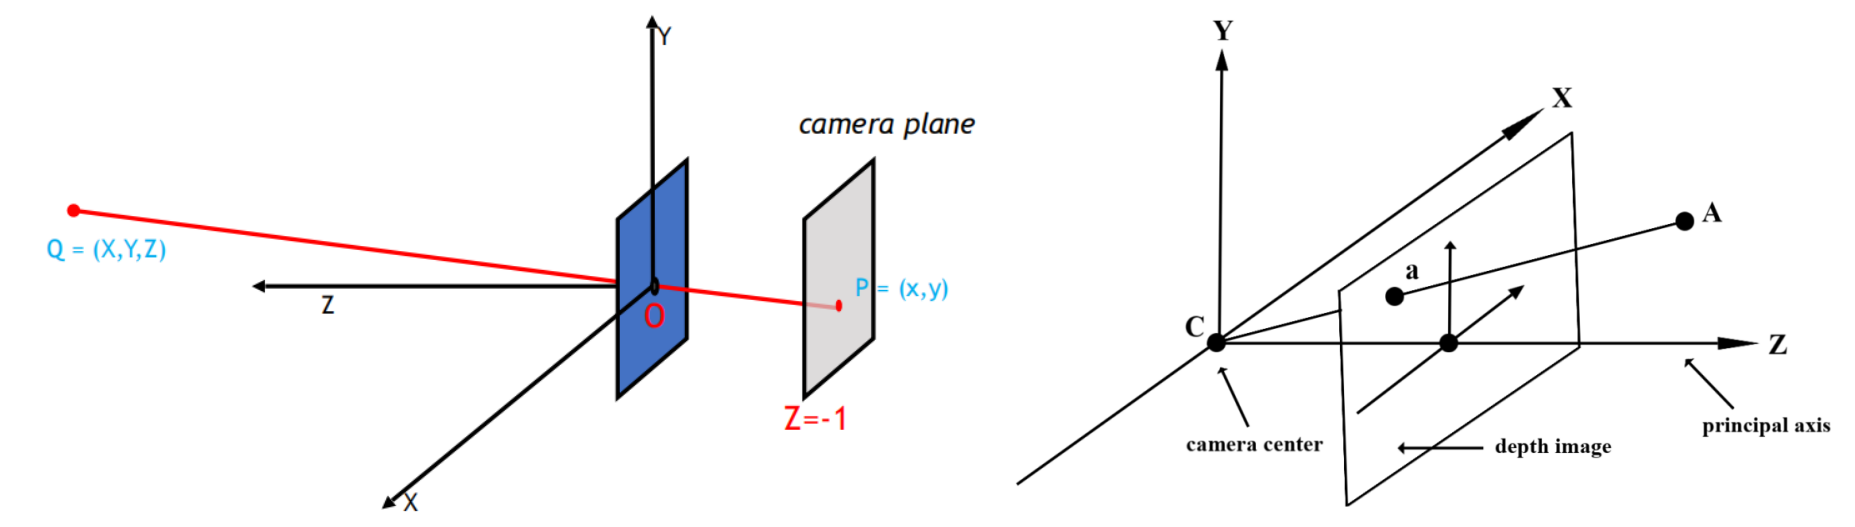
\includegraphics[scale=0.6]{透视投影.png}
\end{figure}

\begin{definition}[射影空间,齐次坐标]
    通过向量空间$V$的原点的直线集合称为射影空间.
    
    在$\R^3$中射影空间可用$\R^2$射影平面表示. 由于三维中通过原点的直线集合可以表示为\\$\{\lambda(x,y,1):\lambda\in\R\}$,
    所以可以用二维点$(x,y)\to(x,y,1)$来表示该直线,故一个平面上的二维点集合可以表示整个三维射影空间.

    类似地,$n$维射影空间为$n-1$维射影平面,$\R^n$中欧式坐标为$(x_1,\cdots,x_{n})$的\textbf{齐次坐标(homogenous coordinates)}为
    $\tsty (\frac{x_1}{x_{n}},\cdots,\frac{x_{n-1}}{x_n},1)$,在射影平面$\R^{n-1}$中表示为$\tsty (\frac{x_1}{x_{n}},\cdots,\frac{x_{n-1}}{x_n})$.
\end{definition}
由于所有位于同一条投影直线(与相机瞳孔相交的“视线”)上的点被投影到图像上的一点,透视投影中成像平面上的全部点构成射影空间,空间向量为$\R^3$,
相机入射瞳孔位于原点,所以透视模型中\textbf{成像平面就是射影平面},透视投影过程就是\textbf{将三维坐标通过齐次坐标转化为二维坐标的过程}.

\paragraph{三维几何变换}
三维几何变换十分类似于二维图像参数几何变换\ref{sec-二维几何变换},将低维向量$(x,y,z)$升维到齐次坐标$(x,y,z,1)$,
于是可以通过齐次坐标完成矩阵的平移操作,便于表示. 
二维几何变换一般形式如下左式,三维几何变换一般形式为右式:
\begin{equation*}
    T_2 = \begin{bmatrix}
        M_2&\bd{t}_2\\
        \bd{0}^T&1
    \end{bmatrix},\qquad T_3 = \begin{bmatrix}
        M_3&\bd{t}_3\\
        \bd{0}^T&1
    \end{bmatrix}
\end{equation*}
其中$M_k\in\R^{k\times k},\bd{t}_k\in\R^k$. 类似二维,$\bd{t}_3$是平移向量,$M_3$用于缩放和旋转.

\subsubsection{透视变换}
将\textbf{三维物体向二维图像的转换}且满足一定的\textbf{几何投影关系},称为\textbf{透视关系}.

\textbf{透视变换}是指对三维物体进行空间变换时,使结果满足透视关系的变换. 通常将针孔相机成像过程称为透视变换,具体过程请见下文坐标系系统.

\paragraph{透视关系(透视变换的特点)}\ \par
1. \textbf{近大远小}:设物体的两端空间坐标为$(X,Y,Z),(X,Y+h,Z)$,则对应的像点为$\tsty(\frac{X}{Z},\frac{Y}{Z})$,
$\tsty(\frac{X}{Z},\frac{Y+h}{Z})$,则成像中物体的高度为$\tsty \frac{Y+h}{Z}-\frac{Y}{Z}=\frac{h}{Z}$,当$Z$增大时,物体变小,反之变大,
所以呈现出近大远小的特点.

2. \textbf{平行线交于一点(消失点)}:设空间中两条平行线为$Q(\lambda) = A+\lambda D,R(\lambda) = B+\lambda D$,则两条线投影后为
\begin{align*}
    q(\lambda)=&\ \left(\frac{A_x+\lambda D_x}{A_z+\lambda D_z}, \frac{A_y+\lambda D_y}{A_z+\lambda D_z}\right)\to \left(\frac{D_x}{D_z},\frac{D_y}{D_z}\right),\quad(\lambda \to\infty),\add\\
    r(\lambda)=&\ \left(\frac{B_x+\lambda D_x}{B_z+\lambda D_z}, \frac{B_y+\lambda D_y}{B_z+\lambda D_z}\right)\to \left(\frac{D_x}{D_z},\frac{D_y}{D_z}\right),\quad(\lambda \to\infty).
\end{align*}

当$D_z\neq 0$时,图像中平行线在无限延长后会在$\tsty (\frac{D_x}{D_z},\frac{D_y}{D_z})$处相交,将该点称为\textbf{消失点}.

当$D_z = 0$时,图像中平行线不会相交,也就是平行于成像平面的平行线,消失点在$(\infty,\infty)$处(例如照片中的两个电线杆无限延长后仍然不会相交).

3. \textbf{平面消失于一条线(消失线)}:设空间中的平面为$\tsty N_xX+N_yY+N_zZ = d\Rightarrow N_x\frac{X}{Z}+N_y\frac{Y}{Z}+N_z=\frac{d}{Z}$,
则成像平面中为一条和$Z$相关的直线$\tsty N_xx+N_yy+N_z = \frac{d}{Z}$,令$Z\to\infty$,则$\tsty N_xx+N_yy+N_z = 0$,称之为\textbf{消失线}.
并且对于空间中平行的平面(改变$d$,不改变法向量$\bd{N}$),消失线相同,说明平行平面会消失于同一消失线处.

当$N_x=N_y=0$时,平面扩张到无限远处,所以没有消失线.

\subsection{相机标定}
\subsubsection{坐标系系统}
\begin{figure}[htbp]
    \centering
    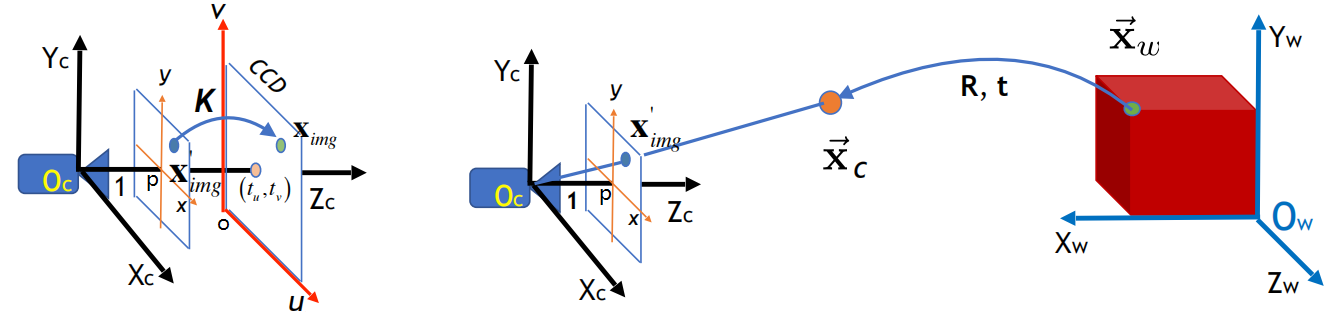
\includegraphics[scale=0.55]{坐标系转换.png}
\end{figure}
1. \textbf{世界坐标系}:三维空间中建立的基准坐标系,用于标记空间点和相机位置,如上图中坐标系$O_w\text{-}X_wY_wZ_w$所示.

2. \textbf{相机坐标系}:以相机中心$O_c$作为原点,从$O_c$出发垂直于成像平面的射线作为主轴$Z_c$,从$O_c$出发与像平面水平平行作为$X_c$轴,
从$O_c$出发与像平面平行且铅垂直作为$Y_c$轴,如上图中坐标系$O_c\text{-}X_cY_cZ_c$所示.

3. \textbf{成像平面坐标系(齐次化坐标系,规范化坐标系)}:成像平面为相机坐标系中$Z_c=1$的平面,记成像平面与$Z_c$的交点为原点$p$,
以像平面水平线和铅垂线分别为$x$轴与$y$轴,上图中坐标系$p\text{-}xy$所示.

4. \textbf{图像坐标系}:原点$o$位于图像的左下角,平行于$x$轴作为$u$轴,平行于$y$轴作为$v$轴,上图中坐标系$o\text{-}uv$所示.

设三维坐标$\bd{x}(X,Y,Z)$,则其对应的齐次坐标为四维坐标$\bd{x'}(X,Y,Z,1)$,
升维以后的齐次坐标能够通过矩阵完成平移操作,便于表示. \textbf{以下坐标定义均为齐次坐标.}

我们记三维空间中物体的世界坐标为$\bd{x}_w$,相机坐标为$\bd{x}_c$(单位:m或mm),成像平面坐标为$\bd{x}'_{img}$,图像坐标为$\bd{x}_{img}$(单位:像素).

则四个坐标系的转换关系如下图所示
\clearpage
\begin{figure}[htbp]
    \centering
    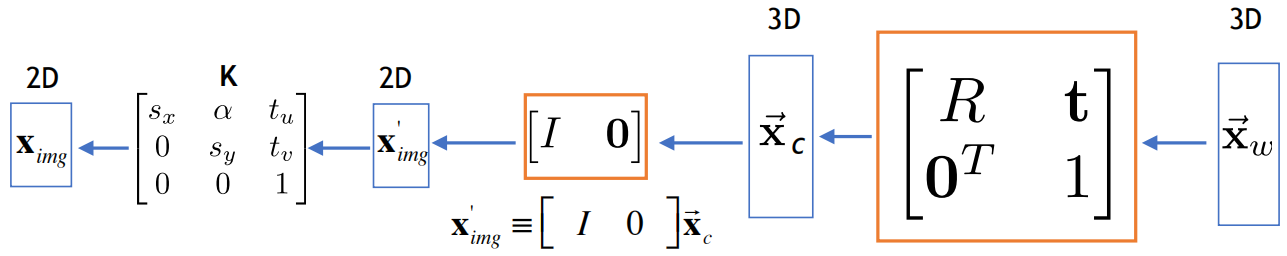
\includegraphics[scale=0.55]{转换坐标.png}
\end{figure}

上图变换主要包含三个矩阵:

1. \textbf{外参矩阵}:$4\times 4$矩阵,包括$3\times 3$的旋转矩阵$R$以及一个$3\times 1$的平移向量$\bd{t}$,\textbf{将世界坐标系转化为相机坐标系},
该矩阵会随着物体或相机的移动而发生变化.

2. \textbf{投影矩阵}:$3\times 4$矩阵,取前三维分量,然后转化为齐次坐标,转化符号记为$\equiv$. 注意,该过程会产生尺度因子$\lambda$,即缩放比例. 如下式所示
\begin{equation*}
    [I\quad 0]\bd{x}_c = \left[\begin{matrix}
        1&0&0&0\\0&1&0&0\\0&0&1&0
    \end{matrix}\right]
    \left[\begin{matrix}
        X_c\\Y_c\\Z_c\\1
    \end{matrix}\right]=\left[\begin{matrix}
        X_c&Y_c&Z_c
    \end{matrix}\right]\equiv\left[\begin{matrix}
        X_c/Z_c\\Y_c/Z_c\\1
    \end{matrix}\right] = \bd{x}'_{img}
\end{equation*}
其中$[I\quad 0]\bd{x}_c = \lambda \bd{x}'_{img}$,$\lambda = 1/Z_c$. 该变换过程就是\textbf{透视投影}.

3. \textbf{内参矩阵$K$}:$3\times 3$矩阵,将像素从成像坐标系转化到图像坐标系中,\textbf{由相机的自有特性决定},不随外部物体变化而变化. 其具体表示如下
\begin{equation*}
    K = \left[\begin{matrix}
        f_x&\alpha&t_u\\
        0&f_y&t_v\\
        0&0&1
    \end{matrix}\right]
\end{equation*}
其中$(t_u,t_v)$表示图像坐标系原点在成像坐标系中所处的位置. 由于需要从单位m或mm转化为像素,
所以还需要$f_x,\ f_y$分别表示沿$x$与$y$轴的缩放比例(相机焦距),由于$o\text{-}uv$不一定正交,所以还存在倾斜因子$\alpha$.

\subsection{相机径向畸变与切向畸变的特点及矫正方法}
在实际应用中,由于光学透镜不是完美的,通过透镜边缘的光线会发生偏转,导致偏离成像位置,发生扭曲,称为光学畸变. 光学畸变主要分为两种:

1. 径向畸变:主要由透镜问题产生,是一种非线性扭曲,畸变程度取决于与主点的距离,光线距离透镜中心越远,畸变效果更为严重. 有枕形畸变和桶形畸变两种.
\begin{figure}[htbp]
    \centering
    \subfigure[桶形畸变]
    {
        \begin{minipage}[b]{0.45\linewidth}
            \centering
            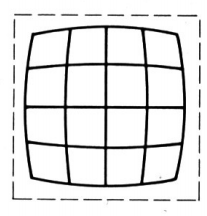
\includegraphics[scale=0.8]{桶形畸变.png}
        \end{minipage}
    }
    \subfigure[枕形畸变]
    {
        \begin{minipage}[b]{0.45\linewidth}
            \centering
            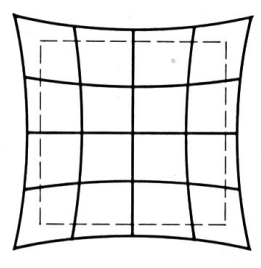
\includegraphics[scale=0.6]{枕形畸变.png}
        \end{minipage}
    }
\end{figure}

2. 在相机安装过程中,光轴与成像平面无法完成平行,导致切向畸变.

两种畸变可用如下模型表示:
\begin{equation*}
    \hspace{-1.4cm}
    \begin{cases}
        x_d-x_c=\overbrace{(x_u-x_c)(1+k_1r^2+k_2r^4+\cdots)}^{\text{径向畸变}}+\overbrace{\left[p_1(r^2+2(x_u-x_c)^2)+2p_2(x_u-x_c)(y_u-y_c)\right](1+p_3r^2+\cdots)}^{\text{切向畸变}}\\
        y_d-y_c=(y_u-y_c)(1+k_1r^2+k_2r^4+\cdots)+\left[p_2(r^2+2(y_u-y_c)^2)+2p_1(x_u-x_c)(y_u-y_c)\right](1+p_3r^2+\cdots)\\
    \end{cases}
\end{equation*}
(下述坐标均在成像坐标系中)其中$(x_u,y_u)$表示理想像素点坐标,$(x_d,y_d)$表示畸变图像点坐标,$(x_c,y_c)$表示畸变中心,$k_n$为镜像畸变系数,$p_n$为切向畸变系数,$r^2=(x_u-x_c)^2+(y_u-y_c)^2$.

令$(x_c,y_c)=(0,0)$,略去部分高阶项,可得简化版畸变模型
\begin{equation}
    \label{eq-简化畸变模型}
    \begin{cases}
        x_d=x_u(1+k_1r^2+k_2r^4)+p_1(r^2+2x_u^2)+2p_2x_uy_u\\
        y_d=y_u(1+k_1r^2+k_2r^4)+p_2(r^2+2y_u^2)+2p_1x_uy_u\\
    \end{cases}
\end{equation}
通过对畸变参数$k_1,k_2,p_1,p_2$进行求解后,反解求得理想像素点坐标$(x_u,y_u)$.

\subsubsection{张氏标定法}
由于世界坐标系可以自由设定,我们不妨取三维平面中的黑白棋盘作为$xOy$平面,则棋盘上的点均有$Z_w = 0$,由相机成像原理可知
\begin{equation*}
    x_{img} = \left[\begin{matrix}
        u\\v\\1
    \end{matrix}\right]\equiv K[R\quad \bd{t}]x_w = K[\bd{r}_1\quad \bd{r}_2\quad \bd{r}_3\quad \bd{t}]\left[\begin{matrix}
        X_w\\Y_w\\0\\1
    \end{matrix}\right] = K[\bd{r}_1\quad \bd{r}_2\quad \bd{t}]\left[\begin{matrix}
        X_w\\Y_w\\1
    \end{matrix}\right] = H\left[\begin{matrix}
        X_w\\Y_w\\1
    \end{matrix}\right]
\end{equation*}
其中$H$矩阵称为棋盘平面与图像平面之间的\textbf{单应性}(Homography)变换矩阵,由于尺度因子的省略,
$H$矩阵对应了相机平面到\textbf{全体同一偏转角度棋盘平面}的一个同态映射.

通过大量的像素坐标以及对应的棋盘格坐标,可建立多个关于$H$的方程组,$H$为$3\times 3$矩阵,
但由于存在一个尺度因子,所以共有$8$个待定参数. 一组对应坐标可以得到两个方程(请见图像对齐\ref{sec-图像对齐}),所以至少$4$组对应坐标,
更多的对应坐标可以通过最小二乘法估计得到$H$矩阵. 下面通过$H$矩阵分别求解内参矩阵$K$,外参矩阵以及径向畸变估计.

\paragraph{估计相机内参矩阵}\del
\begin{equation}
    \label{eq-1}
    H = [\bd{h}_1\quad \bd{h}_2\quad \bd{h}_3] = \lambda K[\bd{r}_1\quad \bd{r}_2\quad \bd{t}]\Rightarrow\begin{cases}
        \bd{r}_1 = \frac{1}{\lambda}K^{-1}\bd{h}_1,\add\\
        \bd{r}_2 = \frac{1}{\lambda}K^{-1}\bd{h}_2.
    \end{cases}
\end{equation}
由于$\bd{r}_1\perp \bd{r}_2,\ ||\bd{r}_1||=||\bd{r}_2||$,于是
\begin{equation}
    \label{eq-2}
    \begin{cases}
        \bd{h}_1^T(K^{-1})^TK^{-1}\bd{h}_2 = 0,\\
        \bd{h}_1^T(K^{-1})^TK^{-1}\bd{h}_1 = \bd{h}_2^T(K^{-1})^TK^{-1}\bd{h}_2,\\
    \end{cases}
\end{equation}
令
\begin{equation*}
    B = (K^{-1})^TK^{-1} = \left[\begin{matrix}
        B_{11}&B_{12}&B_{13}\\
        B_{12}&B_{22}&B_{23}\\
        B_{13}&B_{23}&B_{33}\\
    \end{matrix}\right]
\end{equation*}
由于$B$矩阵是对称阵,所以只需确定下三角部分$6$个参数,令
\begin{equation*}
    \bd{b} = [B_{11}\quad B_{12}\quad B_{22}\quad B_{13}\quad B_{23}\quad B_{33}]^T
\end{equation*}
则上述方程\ref{eq-2}可表示为方程$\begin{cases}
    \bd{v}_{12}^T\bd{b} = 0,\\
    [\bd{v}_{11}^T-\bd{v}_{22}^T]\bd{b} = 0.
\end{cases}$,其中$\bd{v}_{ij}$由$H$矩阵确定,具体形式请见\textit{知乎文章}\footnote{\url{https://zhuanlan.zhihu.com/p/136827980}}.
由于每种不同角度的棋盘图像可以确定不同的$H$矩阵,从而确定$\bd{v}_{ij}$,
于是每张不同角度的棋盘图像可以确定两个关于$\bd{b}$的方程,总共有$6$个待定参数,所以需要至少$3$张不同角度的棋盘才能唯一确定内参矩阵.

\subsubsection{估计相机外参矩阵}
有了内参矩阵$K$以后,我们通过式\ref{eq-1}可知
\begin{equation*}
    \lambda[\bd{r}_1\quad \bd{r}_2\quad \bd{t}] = K^{-1}[\bd{h}_1\quad \bd{h}_2\quad \bd{h}_3]
\end{equation*}
则
\begin{equation*}
    \begin{cases}
        \lambda = ||K^{-1}\bd{h}_1||_2 = ||K^{-1}\bd{h}_2||_2,\\
        \bd{t} = K^{-1}\bd{h}_3/\lambda,\\
        \bd{r}_1 = K^{-1}\bd{h}_1/\lambda,\\
        \bd{r}_2 = K^{-1}\bd{h}_2/\lambda,\\
        \bd{r}_3=\bd{r}_1\times \bd{r}_2.
    \end{cases}
\end{equation*}
其中$||\cdot||_2$为$\ell_2$范数(欧式范数),于是外参矩阵为$[R\quad \bd{t}] = [\bd{r}_1\quad \bd{r}_2\quad \bd{r}_3\quad \bd{t}]$.

在实际应用中,由于数据中存在噪音,$R$矩阵不一定完全满足旋转矩阵的性质,所以通常使用奇异值分解求解$R$.

\subsubsection{最大似然估计畸变参数}
在实际标定过程中,一般存在大量标定图片同时对参数进行估计,这时可以使用最大似然估计对上述算法进行优化. 假设有$n$张标定图片,每张图片中都有$m$个棋盘格角点,且棋盘格大小一致,棋盘中角点相对位置相同. 利用平方损失函数,构造最小化风险函数如下
\begin{equation*}
    \min_{K,\bd{k},R,\bd{t},\lambda}\frac{1}{n}\sum_{i=1}^n\sum_{j=1}^m\left|\left|x_{ij}-x'(K,\bd{k},R_i,\bd{t}_i,\lambda_i,X_{j})\right|\right|^2
\end{equation*}
其中$K$为内参矩阵,$\bd{k}$为径向畸变参数,$[R_i\quad \bd{t}_i]$为第$i$张图像对应的外参矩阵,$\lambda_i$为第$i$张图像对应的尺度因子,第$i$张图像中与棋盘中第$j$个角点坐标$X_{j}$对应的图像坐标为$x_{ij}$,$x'(\cdot)$为根据棋盘中角点坐标$X_{j}$以及由该图片对应的外参数矩阵$[R_i\quad \bd{t}_i]$、尺度因子$\lambda_i$及内参矩阵和径向畸变,预测得到的图像像素坐标.

\subsection{双目立体视觉}
\subsubsection{三角测量}
假设有两个内参已知的相机,从两个不同角度拍摄同一物体,物体上的某点$\bd{x}_w(X,Y,Z)$,在两个相机拍摄的图像上对应坐标分别为$\bd{x}^{(1)}(x_1,y_1),\bd{x}^{(2)}(x_2,y_2)$,
则$\begin{cases}
    \bd{x}^{(1)} \equiv P^{(1)}\bd{x}_{w}\\
    \bd{x}^{(2)} \equiv P^{(2)}\bd{x}_{w}
\end{cases}$. \\
假设$P^{(1)},P^{(2)}$已知,求世界坐标$\bd{x}_{w}$,用最小二乘法估计世界坐标$\bd{x}_w$,最优化问题如下所示
\begin{align*}
    \hat{\bd{x}}_{w} = \argmin_{\bd{x}_w}&\ \quad\sum_{k=1}^2||\bd{x}^{(k)}-P^{(k)}\bd{x}||_2^2\\
    \text{其中}\quad ||\bd{x}^{(k)}-P^{(k)}\bd{x}_w||_2^2 \equiv&\ \left[x - \frac{P_{11}X+P_{12}Y+P_{13}Z+P_{14}}{P_{31}X+P_{32}Y+P_{33}Z+P_{34}}\right]^2 + 
    \left[y - \frac{P_{21}X+P_{22}Y+P_{23}Z+P_{24}}{P_{31}X+P_{32}Y+P_{33}Z+P_{34}}\right]^2
\end{align*}
上式右边$x,y,P$省略了下标,可以表示$x_1,y_1,P^{(1)}$或者$x_2,y_2,P^{(2)}$. 称$||\bd{x}^{(k)}-P^{(k)}\bd{x}_w||_2^2$为\textbf{重建误差(Reprojection error)}.
推导重建误差的方法就是将世界坐标$\bd{x}_w$通过$P^{(k)}$转化为齐次坐标,删去第三维分量后,再求与$\bd{x}$的欧氏距离平方后的结果.

\subsection{立体重建(3D重建)}
\textbf{立体重建(Stereo reconstruction, 3D reconstruction)}指根据多张不同位置相机的拍摄同一物体的图像,获得该物体的世界坐标.

单目相机也就是相机标定所用的,只需一个相机和标定的点对,可以求出相机的内参与外参,但是无法获得物体相对相机的距离,而通过已知内参的双目相机,
可以求出物体到相机的距离,从而求出物体的世界坐标,进行立体重建.

\subsubsection{双目相机}
\textbf{双目相机(矫正相机,Rectified cameras)}:沿$x$轴方向彼此平行、主轴方向且内参基本相同的两个相机. 
若相机内参不同,则需进行\textbf{相机校准},使得两个相机的缩放比例上相同. 如下图所示\del\del
\begin{figure}[htbp]
    \centering
    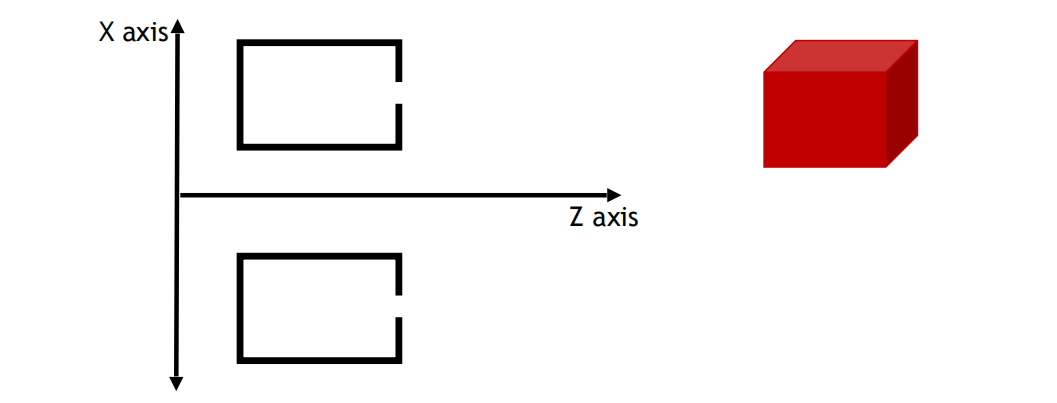
\includegraphics[scale=0.5]{双目相机.png}
\end{figure}

设双目相机在$x$轴方向上的距离为$t_x$,称为\textbf{基线(baseline)}. 将相机编号为1,2,
以相机1作为坐标系原点,空间中物体位于$\bd{x}_w(X,Y,Z)$,
在两个相机上的像点分别为$\bd{x}^{(1)}(x_1,y_1),\bd{x}^{(2)}(x_2,y_2)$,由成像原理可知:\del\del
\begin{align}
    \label{eq-双目相机}\bd{x}^{(1)}\equiv [I\quad \bd{0}]\left[\begin{matrix}
        \bd{x}_w\\ 1
    \end{matrix}\right],&\ 
    \bd{x}^{(2)}\equiv [I\quad \bd{t}_x]\left[\begin{matrix}
        \bd{x}_w\\ 1
    \end{matrix}\right],
    \\
    \nonumber\begin{bmatrix}
        x_1\\y_1
    \end{bmatrix}\equiv \begin{bmatrix}
        1&0&0&0\\
        0&1&0&0\\
        0&0&1&0
    \end{bmatrix}\begin{bmatrix}
        X\\Y\\Z\\1
    \end{bmatrix} = \begin{bmatrix}
        X\\Y\\Z
    \end{bmatrix},&\ 
    \begin{bmatrix}
        x_2\\y_2
    \end{bmatrix}\equiv \begin{bmatrix}
        1&0&0&t_x\\
        0&1&0&0\\
        0&0&1&0
    \end{bmatrix}\begin{bmatrix}
        X\\Y\\Z\\1
    \end{bmatrix} = \begin{bmatrix}
        X+t_x\\Y\\Z
    \end{bmatrix},\ 
\end{align}
于是$x_1 = \frac{X}{Z}, x_2 = \frac{X+t_x}{Z}, y_1=y_2=\frac{Y}{Z}$,
则$x_2-x_1 = \frac{t_x}{Z}\Rightarrow Z = \frac{t_x}{x_2-x_1}=\frac{t_x}{d}$.\add
其中$d=x_2-x_1$称为\textbf{视差(disparity)}
表示同一物体在两个图像上对应像素点之间的$x$轴方向距离,$Z$称为\textbf{景深(depth)}表示物体距离相机的距离,$t_x$为\textbf{基线(baseline)}.
如果我们得到了$d$,\add 由于$t_x$已知,于是可得景深$Z$.(\textbf{上述推导中默认了内参矩阵$K$为单位阵,否则表达式中还需加入焦距$Z = \frac{ft_x}{d}$})

\subsubsection{视差估计}
由于假设相机位于统一水平面上,所以拍摄出的图像仅在$x$轴方向上发生小范围移动(近处移动大、远处移动小),使用\textbf{横向滑动窗口方法匹配相似点}. 
设两个相机拍摄统一物体得到的图像分别为$f,g$,
对于$f$中的像素点$(x_1,y_1)$,只需在$g$中$y=y_1$的水平线上寻找相似点,若$(x_1,y_1)$与$(x_1+d,y_1)$周围图像近似,则可认为$(x_1,y_1)$处的视差为$d$.
用$NCC$判断相似性大小.

设总共有$D$种可能的视差,窗口大小为$k\times k$,具体步骤如下:
\begin{enumerate}
    \item 考虑$f$中的像素点$(x_1,y_1)$,以$(x_1,y_1)$为中心大小为$k\times k$的窗口,以窗口内的像素值集合$X$作为$(x_1,y_1)$处的特征描述子;
    \item 选取可能的视差$d\in D$,取$g$中以$(x_1+d,y_1)$为中心的大小为$k\times k$的特征描述子$Y$;
    \item 计算$NCC(X,Y)$(归一化互相关),若NCC相似度大于最优值,记录视差$d$;
    \item 重复步骤2,3,知道遍历完所有视差$d$.
    \item 用最终记录的最优视差$d$作为$(x_1,y_1)$处的视差,计算出该处的景深$Z = \frac{t_c}{d}$.
\end{enumerate}
\begin{figure}[htbp]
    \vspace{-0.5cm}
    \centering
    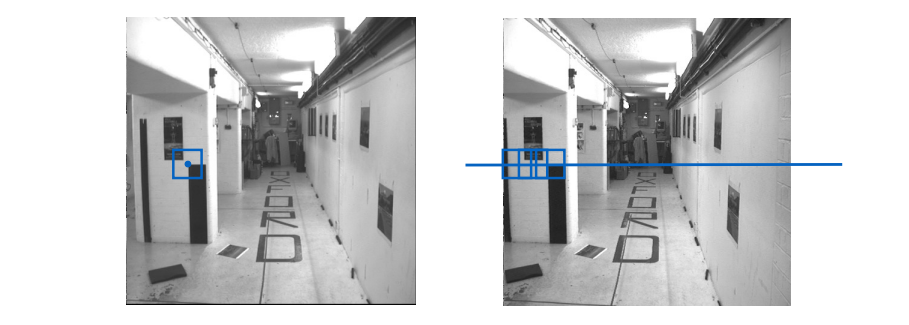
\includegraphics[scale=0.6]{移动窗口视差估计.png}
\end{figure}

另一种描述方法:求出特征描述子张量$M\times N\times K^2$,表示每个像素点对应的窗口特征描述子,
\textbf{NCC成本张量(NCC cost volumne)}大小为$M\times N\times D$,其中$(x,y,d)$表示$f(x,y),g(x+d,y)$对应特征描述子的NCC相似度,
最后对$NCC$成本张量的第三维求最大值即可得到每个像素点处的视差. 如下图所示:\del
\begin{figure}[htbp]
    \hspace{-0.7cm}
    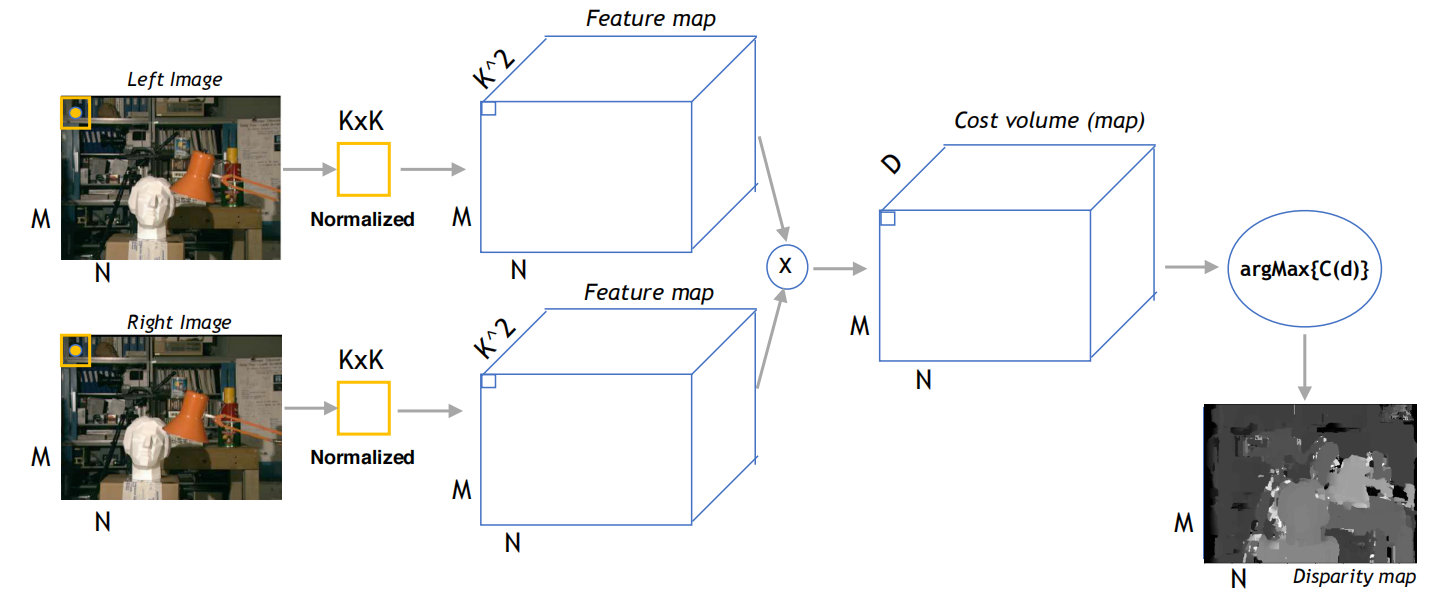
\includegraphics[scale=0.6]{视差估计.png}
\end{figure}
\paragraph{图像校正}即使两个相机在同一平面上拍摄时,拍摄出的图像仍可能无法保证$x$轴是对齐的,
先找到搜索点的\textbf{对极线},将对极线旋转至与$x$轴平行,再做视差估计(对极线内容请见下文)

总的来说,立体重建分为四步:\textbf{1. 相机标定;2. 图像校正;3. 计算视差;4. 估计景深}.
\subsection{对极几何}
\subsubsection{基本概念}
\textbf{基线}:两个相机入射瞳孔光心构成的连线;\par
\textbf{极点}:基线与成像平面的交点$e,e'$;\par
\textbf{对应点}:三维空间中点$X$在两个不同成像平面上的像点$\bd{x},\bd{x}'$;\par
\textbf{极线}:像点与极点构成的直线,$l$为左极线,$l'$为右极线.\par
\textbf{对极约束}:将对应点搜索问题转化为对极线上搜索问题.(可以解决视差估计中图像不对齐的的搜索问题)\par
\textbf{性质}:三维空间中物体$X$移动,只有极线和成像点发生变化. 左平面上像点$\bd{x}$可唯一对应一条右极线$l'$,且右像点$\bd{x}'$一定落在$l'$上(反之亦然).
固定相机位置,无论如何移动$\bd{X}$,均有左极线一定过左极点$e$,右极线一定过右极点$e'$.\del
\begin{figure}[htbp]
    \centering
    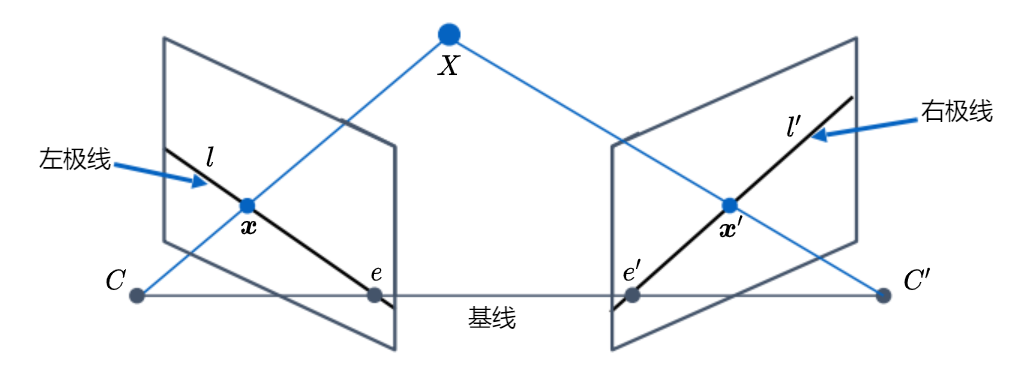
\includegraphics[scale=0.35]{对极几何.png}
\end{figure}
\subsubsection{本质矩阵与基础矩阵}  % 重点
设空间中物体位于$\bd{x}_w$,由相机成像原理可知
\begin{equation*}
    \bd{x}^{(1)}_{img}\equiv K_1[R\quad \bd{t}_1]\bd{x}_w,\quad
    \bd{x}^{(2)}_{img}\equiv K_2[R\quad \bd{t}_2]\bd{x}_w
\end{equation*}
先假设内参矩阵$K_1,K_2$为单位阵,以相机1作为坐标系原点,$\bd{x}_w'$为$\bd{x}_w$的齐次坐标,则
\begin{equation*}
    \bd{x}^{(1)}_{img}\equiv [I\quad \bd{0}]\bd{x}_w' = \bd{x}_w,\quad \bd{x}^{(2)}_{img}\equiv [R\quad \bd{t}]\bd{x}_w'=R\bd{x}_w+\bd{t},
\end{equation*}
\textit{双目相机原理式(\ref{eq-双目相机})是上式的特殊形式.}

将左式代入右式可得$\bd{x}^{(2)}_{img}\equiv R\bd{x}^{(1)}_{img} + \bd{t}$,再左右作外积$\bd{x}^{(2)}_{img}\cdot \bd{t}$可得
\begin{equation*}
    \bd{x}^{(2)}_{img}\cdot t\times R\bd{x}^{(1)}_{img} = \bd{0}
\end{equation*}
由于外积可写做矩阵乘法形式:$\bd{t}\times R = [\bd{t}]_{\times}R$,其中$[\bd{t}]_{\times} = \begin{bmatrix}
    0&-t_z&t_y\\
    t_z&0&-t_x\\
    -t_y&t_x&0
\end{bmatrix}$称为$\bd{t}$的\textbf{反对称矩阵}. 由于向量内积可以表示为矩阵乘法形式$\bd{x}\cdot \bd{y} = \bd{x}^T\bd{y}$,
于是可以进一步改写上式:
\begin{equation*}
    \bd{x}^{(2)T}_{img}[t]_{\times}R\bd{x}^{(1)}_{img}=  \bd{0}\Rightarrow \bd{x}^{(2)T}_{img}E\bd{x}^{(1)}_{img} = \bd{0}
\end{equation*}
其中$E = [t]_{\times}R$称为\textbf{本质矩阵},由相机的相对位置决定.

当$K_1,K_2$为一般情况时,则
\begin{equation*}
    \bd{x}^{(1)}_{img}\equiv K_1\bd{x}_w,\quad \bd{x}^{(2)}_{img}\equiv K_2[R\quad \bd{t}]\bd{x}_w
\end{equation*}
经过上述类似推导可得
\begin{equation*}
    \bd{x}^{(2)T}_{img}K_2^{-1}[t]_{\times}RK_1^{-1}\bd{x}^{(1)}_{img} = \bd{0}\Rightarrow \bd{x}^{(2)T}_{img}F\bd{x}^{(1)}_{img} = \bd{0}
\end{equation*}
其中$F = K_2^{-1}[t]_{\times}RK_1^{-1}$称为\textbf{基础矩阵}.

\paragraph{极线与极点性质解释}以本质矩阵为例,\add 假设固定$\bd{x}^{(1)}_{img}$,令$\bd{l} = E\bd{x}^{(1)}_{img}$,于是$\bd{x}^{(2)T}_{img}\bd{l} = \bd{0}$,
则$\bd{l}$确定了相机2的成像平面上的一条直线,\add 这就是由$\bd{x}^{(1)}_{img}$对应的极线$E\bd{x}^{(1)}_{img}$.
类似地,固定$\bd{x}^{(2)}_{img}$也可以在相机1的成像平面上导出对应的极线$E^T\bd{x}^{(2)}_{img}$(对极线).

令$\bd{e}' = \bd{t}$,则$\bd{e}'^TE= \bd{t}^T[t]_{\times}R = \bd{t}\cdot\bd{t}\times R = \bd{0}$,于是$\bd{e}'^TE\bd{x}^{(1)}_{img} = \bd{e}'^T\bd{l} = \bd{0},\ (\forall \bd{l})$,
所以相机2的全部极线都经过点$\bd{e}'$,则$\bd{e}'$是相机2的极点. 类似地,令$\bd{e} = R^T\bd{t}$,可得$\bd{e}$是相机1的极点.

在内参$K_1,K_2$为一般情况下,也就是对于基础矩阵$F$,也有对极线$F\bd{x}^{(1)}_{img},F^T\bd{x}^{(1)}_{img}$,
极点满足$e'^TF = \bd{0},\ E\bd{e} = \bd{0}$,由于$F\in\R^{3\times 3}$,所以$F$的阶数\textbf{应该为$2$阶}.(这个性质常用于在计算中校准$F$矩阵)

\paragraph{8点法估计$F$矩阵}(复习内容中没有包含,大致讲解原理)
若不清楚相机内参数 $K_1,K_2,R,t$ 则可通过对应点直接反解 $F$ 矩阵. 
对应点满足的方程为 $x'^T F x = 0$,其中 $x'$ 与 $x$ 对应. 由于 $F$ 的自由度为 $8$,每个对应点只能提供一个方程,
所以至少需要 $8$ 个对应点. 也可使用最小二乘法或SVD分解求解.

求解出的$F$的秩可能不为$2$,通过SVD分解令第三个特征值为$0$,再恢复$F$矩阵.

\subsection{运动场与光流场}
\subsubsection{运动场}  % 重点
令空间中物体位于$P(X,Y,Z)$,对应的像点为$p(x,y,f)$,其中$f$表示相机焦距. 由针孔成像原理,有$p = \frac{f}{Z}P$.

考虑物体位置随时间发生变换,则$P=P(t),p=p(t)$,设空间中物体的位移相对速度为$\frac{\d P}{\d t} = V = -\bd{t}-\bd{w}\times P$,
其中$\bd{t} = (t_x,t_y,t_z)^T$为平移向量,$\bd{w} = (w_x,w_y,w_z)^T$为旋转向量. \add 
则空间相对速度的各维度分量为
\begin{equation}
    \label{eq-空间相对速度}
    \begin{cases}
        V_x = -t_x - w_yZ+w_zY,\\
        V_y = -t_y - w_zX + w_xZ,\\
        V_z = -t_z - w_xY + w_yX.
    \end{cases}
\end{equation}
像点相对速度为$\bd{v} = \frac{\d p}{\d t} = \frac{\d\frac{fP}{Z}}{\d t} = \frac{fVZ-fPV_z}{Z^2} = f\frac{V}{Z}-p\frac{V_z}{Z}$,
令
\begin{equation}
    \label{eq-像点相对速度}
    \begin{cases}
        u = \bd{v}_x = f\frac{V_x}{Z} - x\frac{V_z}{Z},\add\\
        v = \bd{v}_y = f\frac{V_y}{Z} - y\frac{V_z}{Z},\add\\
        \bd{v}_z = f\frac{V_z}{Z} - f\frac{V_z}{Z} = 0.
    \end{cases}
\end{equation}
将式(\ref{eq-空间相对速度})代入式(\ref{eq-像点相对速度})中,并利用$Y = \frac{Z}{f}y,X=\frac{Z}{f}x$可得\textbf{运动场方程(Motion Field)}
\begin{align*}
    \begin{cases}
        u = \overbrace{\frac{xt_z-ft_x}{Z}}^{\text{平移部分}}+\overbrace{\frac{x_y}{f}w_x - (f+\frac{x^2}{f})w_y+yw_z}^{\text{旋转部分}},\\
        v = \frac{yt_z-ft_y}{Z}+(f+\frac{y^2}{f})w_x-\frac{x_y}{f}w_y+xw_z.
    \end{cases}
\end{align*}
上述方程由两部分构成,一个为平移部分,另一个为旋转部分,注意到旋转部分与深度$Z$无关. 运动场方程还可以写成矩阵的形式
\begin{equation*}
    \begin{bmatrix}
        u\\v
    \end{bmatrix} = \frac{1}{Z}\begin{bmatrix}
        -f&0&x\\0&-f&y
    \end{bmatrix}\begin{bmatrix}
        t_x\\t_y\\t_z
    \end{bmatrix}+\begin{bmatrix}
        \frac{xy}{f}&-f-\frac{x^2}{f}&y\add\\
        f+\frac{y^2}{f}&-\frac{xy}{f}&x
    \end{bmatrix}\begin{bmatrix}
        w_x\\w_y\\w_z
    \end{bmatrix} =: \frac{1}{Z}A\bd{t} + B\bd{w}
\end{equation*}

\paragraph{平移运动场(Translational field)}
只考虑物体做平移运动,令$\bd{w} = \bd{0}$,当$t_z\neq 0$时,有
\begin{equation*}
    \begin{cases}
        u = \frac{t_z}{Z}(x-\frac{ft_x}{t_z}),\add\\
        v = \frac{t_z}{Z}(y-\frac{ft_y}{t_z}).
    \end{cases}
\end{equation*}
于是上述方程有不动点$(\frac{ft_x}{t_z}, \frac{ft_y}{t_z})$,该点称为\textbf{FOE(focus of expansion)}点,表示物体做带有深度变换的平移时,
像点运动的相对速度向量MF$\bd{v}$会以FOE点作为中心,向外呈放射状,或者向内呈收缩状.

当$t_z = 0 $时,有
\begin{equation*}
    \begin{cases}
        u = -\frac{ft_x}{Z},\add\\
        v = -\frac{ft_y}{Z}.
    \end{cases}
\end{equation*}
于是FOE点位于$(\infty, \infty)$,相对速度向量MF相互平行.

仅考虑平移运动时,相对速度向量MF都与深度$Z$成反比关系.
\subsubsection{光流场}
\begin{definition}[光流向量]
    光流场是图像中亮度模式的表观运动.
\end{definition}
在理想条件下,光流场与运动场相同. 需要注意的是,如果物体没有运动,光照的变换也有可能使光流场发生变换. 所以需要加入以下三条\textbf{光流约束}:
\begin{enumerate}
    \item \textbf{亮度恒常性(Brightness constancy)}:两个相邻的亮度不会发生变化.
    \item \textbf{微小运动(Small motion)}:物体运动距离不大.
    \item \textbf{空间相关性(Spatial coherence)}:相邻点具有相同的运动方向.
\end{enumerate}
\subsubsection{Lucas-Kanade光流算法}  % 重点
Lucas-Kanade光流算法也简称为L-K光流算法,设图像为$I(\cdot)$,由亮度恒常性可得
\begin{align*}
    &\ I(x,y,t-1) = I(x+u(x,y),y+v(x,y),t)\approx u(x,y)I_x+v(x,y)I_y+I(x,y,t)\\
    \Rightarrow&\ uI_x+vI_y+I_t\approx 0
\end{align*}
令$\Omega$为$(x_0,y_0)$的一个小邻域,内部点具有相同的光流向量,定义均方损失函数,则
\begin{align*}
    E(u,v) =&\ \sum_{(x,y)\in\Omega}w(x,y)(uI_x+vI_y+I_t)^2\\
    =&\ \sum_{(x,y)\in\Omega}w(x,y)\left(\begin{bmatrix}
        I_x&I_y&I_t
    \end{bmatrix}\begin{bmatrix}
        u\\v\\1
    \end{bmatrix}\right)^2\\
    =&\ \sum_{(x,y)\in\Omega}w(x,y)\begin{bmatrix}
        u&v&1
    \end{bmatrix}\begin{bmatrix}
        I_x^2&I_xI_y&I_xI_t\\
        I_yI_x&I_y^2&I_yI_t\\
        I_tI_x&I_tI_y&I_t^2
    \end{bmatrix}\begin{bmatrix}
        u\\v\\1
    \end{bmatrix}
\end{align*}
其中$w(x,y)$表示Gauss核$G_\sigma$,于是
\begin{align*}
    \frac{\partial E(u,v)}{\partial (u,v)} = 0
    \Rightarrow&\ 
    \sum_{(x,y)\in\Omega}w(x,y)\begin{bmatrix}
        I_x^2&I_xI_y\\
        I_yI_x&I_y^2
    \end{bmatrix}\begin{bmatrix}
        u\\v
    \end{bmatrix} = -\sum_{(x,y)\in\Omega}w(x,y)\begin{bmatrix}
        I_x&I_t\\I_y&I_t
    \end{bmatrix}\\
    \Rightarrow&\ 
    G_\sigma*\begin{bmatrix}
        I_x^2&I_xI_y\\
        I_yI_x&I_y^2
    \end{bmatrix}\begin{bmatrix}
        u\\v
    \end{bmatrix} = -G_\sigma*\begin{bmatrix}
        I_x&I_t\\I_y&I_t
    \end{bmatrix}
\end{align*}
通过最小二乘法即可解出$(u,v)$,得到$(x_0,y_0)$处的光流向量.
\paragraph{Coarse-to-fine光流估计}
Coarse-to-fine光流估计是对L-K算法的改进,由于需要满足亮度恒常性条件,所以物体的移动不能太大,对两幅图像$I(x,y,t-1)$和$I(x,y,t)$来那个幅图像
利用Gauss金字塔进行缩放,对每一层处对应图像做L-K算法,选取效果最好的一组. 如下图所示:
\begin{figure}[htbp]
    \centering
    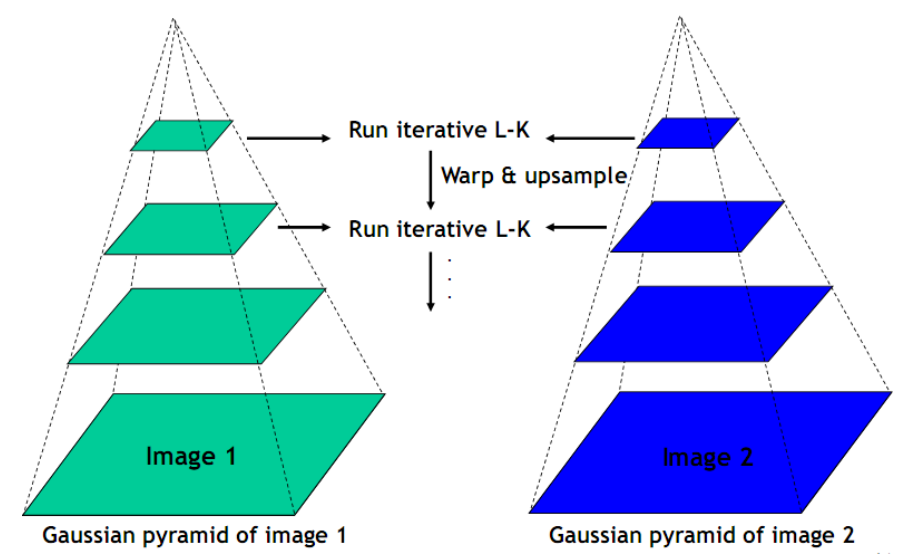
\includegraphics[scale=0.7]{coarse_to_fine光流估计.png}
\end{figure}
\end{document}

% 重点
% 卷积与互相关,双边滤波器,下采样与上采样
% Canny边缘检测,Harris角点检测,RANSAC算法
% 相机标定,视差估计,本质矩阵与基础矩阵,运动场,Lucas-Kanade光流算法
%